%! TeX program = pdflatex
\documentclass{report}
\usepackage[english]{babel}
\usepackage[utf8]{inputenc}
\usepackage{amsmath}
\usepackage{amssymb}
\usepackage{graphicx}
% \usepackage{natbib}
\usepackage{pgf}
% \usepackage{url}
\usepackage{algorithm}% http://ctan.org/pkg/algorithms
\usepackage{algpseudocode}% http://ctan.org/pkg/algorithmicx
% \usepackage{tikz-cd}
\usepackage{listings}
% \usepackage{xcolor}
% \usepackage[colorlinks, linkcolor = blue, citecolor = magenta]{hyperref}
\usepackage{tikz}
% % \usepackage{minted}
\usepackage{float}
% \usetikzlibrary{shapes, arrows, positioning}
% \lstset{ 
%     language=Python,                 % the language of the code
%     basicstyle=\ttfamily\small,      % the size of the fonts that are used for the code
%     numbers=left,                    % where to put the line-numbers
%     numberstyle=\tiny\color{gray},   % the style that is used for the line-numbers
%     stepnumber=1,                    % the step between two line-numbers. If it's 1, each line will be numbered
%     numbersep=5pt,                   % how far the line-numbers are from the code
%     backgroundcolor=\color{white},   % choose the background color. You must add \usepackage{color}
%     showspaces=false,                % show spaces adding particular underscores
%     showstringspaces=false,          % underline spaces within strings
%     showtabs=false,                  % show tabs within strings adding particular underscores
%     frame=single,                    % adds a frame around the code
%     rulecolor=\color{black},         % if not rolframe-color may be changed on line-breaks within not black text (e.g. comments (green here))
%     tabsize=4,                       % sets default tabsize to 4 spaces
%     captionpos=b,                    % sets the caption-position to bottom
%     breaklines=true,                 % sets automatic line breaking
%     breakatwhitespace=false,         % sets if automatic breaks should only happen at whitespace
%     title=\lstname,                  % show the filename of files included with \lstinputlisting; also try caption instead of title
%     keywordstyle=\color{blue},       % keyword style
%     commentstyle=\color{green},      % comment style
%     stringstyle=\color{red},         % string literal style
%     escapeinside={\%*}{*)},          % if you want to add LaTeX within your code
%     morekeywords={*,...} 
% }            % if you want to add more keywords to the rol\newenvironment{notation}
\newtheorem{remark}{Remark}
\newtheorem{definition}{Definition}
\newtheorem{property}{Property}

\newcommand{\pder}[2]{\frac{\partial #1}{\partial #2}}

\title{Electrical grid simulation in the COLMENA framework}
\author{Pablo de Juan Vela $^{1}$ \\
        \small $^{1}$eRoots, Barcelona, Spain \\
}
\date{\today}

\usepackage[style=ieee]{biblatex}
\addbibresource{ref.bib}

\begin{document}
\maketitle

\chapter{Initial Documentation}
%\section[short]{Additional and Alternative Formulation}

\subsection{Devices}

In our modelling, we consider an electrical device as the representation of the physical capabilities of an element of the grid. Let's first define the concept of a simple device. A simple device is a device with a state variable $x \in \mathbb{R}^n$, an algebraic variable $y \in \mathbb{R}^m$, a set of parameters $p \in \mathbb{R}^k$ and a set of acceptable roles $\mathcal{R}(d)$. The set of acceptable roles is limited by the capabilities of the device and also by the state and algebraic variables available to the device. So we have that:

\begin{equation}
    \mathcal{R}(d) = \{ r_i := (f_{r_i}(x,y), g_{r_i}(x,y)) | i \in \}
\end{equation}

Additionally a simple device can only have a single active role at a time. This type of device is meant as a building block for more complicated devices and is a useful tool to see the direct link between the active roles and the final DAE of an agent. In this case we have that if role $r$ is active at a certain time then the DAE is the following.

\begin{align}
    \dot{x} &= f_r(x,y)\\
    0 &= g_r(x,y) 
\end{align}

While the whole DAE for every timesteps get the following form:

\begin{align}
    \dot{x} &= \sum_{r_i \in \mathcal{R}(d)} u_{r_i}(t) f_{r_i}(x,y)\\
    0 &= \sum_{r_i \in \mathcal{R}(d)} u_{r_i}(t) g_{r_i}(x,y)
\end{align}


Lets take for example a generator device. The generator has at least the states $\delta$ the rotor angle and $\omega$ the rotor's speed. An acceptable role for a generator needs to define the differential equations for this variables and take into account the dependencies into the definition of $f(x,y)$ and $g(x,y)$.

\subsection{Edges}

Previously, we defined an environment as a set af agents that can share information \ref{environment}. This information is exchanged through edges. The edge is composed of a logger, and a dashboard. The logger stores the data inputed from the different agents and the dahsboard stores the data that edge outputs that is available to the agents. To define the behaviour of the edge and how the data stored evolves we need to work with different parts:

\begin{itemize}
    \item A measure: the type of value that the agents publish to the logger.
    \item An update function to filter the logger overtime.
    \item A KPI of the form $f(logger)$ to publsih to the dashboard.
\end{itemize}

These three elements along with the environment definition define the behaviour and the interactions of the edge. 

\subsection{Behavioural Roles}

One way to think about the roles of an agent is to think about the DAE that this role represents. In this proposed definition the active role completely defines the evolution of the agents state $x$ by a set of differeential equations $f(x,y)$ and algebraic rquations $g(x,y)$.
\begin{definition}
    Let $A$ a role belonging to the role set $\mathcal{R}(d)$ of the agent $d$. Then $A := \{ f_{A|I}(x,y), g_{A|I}(x,y) | I \in  \mathcal{R}(d)\} $ such that when the agent $d$ takes on the role $A$ the agent behavior is described by this DAE:
    \begin{align}
        \dot{x}_{A} &= \sum_{A_i \in \mathcal{R}(d)} u_{A_i}(t) f_{A|A_i}(x,y)\\
        0 &= \sum_{A_i \in \mathcal{R}(d)} u_{A_i}(t) g_{A|A_i}(x,y) \qquad \forall A_i
    \end{align}

    \begin{equation}
        u_A(t) = \begin{cases}
            1 & \text{if role is A} \\
            0 & \text{if else} 
        \end{cases}
    \end{equation}
\end{definition}

This role definition lends itself to combining multiple roles. We can add the differential equations of the active roles and define  
a new DAE that takes into account multiple roles. Let's take for exampla an agent $a$ at time $t$ with active roles $A,B,C \in \mathcal{d}$. Then the DAE at time $t$ is defined as follows:

Finally, we can express the DAE $\forall t \in \mathcal{T}$ combining the previous deifnitions as follows
\begin{align}
    \dot{x} &= \sum_{A_i \in \mathcal{R}(d)}u_{A_i}(t)\sum_{A_j \in \mathcal{R}(d)} f_{A_i|A_j}(x,y)\\
    0 &= \sum_{A_i \in \mathcal{R}(d)}u_{A_i}(t)\sum_{A_j \in \mathcal{R}(d)} g_{A_i|A_j}(x,y)\\
\end{align}

In this case, we can see that the system is heavily dependent on the interactions between the different roles. However, if we consider the roles to be independent from each other ($f_{A_i|A_j}(x,y) = 0 \forall i \neq j$) we can simplify the DAE and get a DAE with the following equations:

\begin{align}
    \dot{x} &= \sum_{A_i \in \mathcal{R}(d)} u_{A_i}(t)f_{A_i|A_i}(x,y)\\
    0 &= \sum_{A_i \in \mathcal{R}(d)}u_{A_i}(t)g_{A_i|A_i}(x,y)\\
\end{align}

\subsection{Restarting roles}

As we can see, properly defining the interactions between the roles is a critical part of the modelization. More specifically, defining the appropriate behaviour of the device's states when swapping the roles can be challenging. For this purpose, we define a role that restarts the state from an initial point $x_0$ after a role swap. This new initial state is defined by the function $x_0:= f_0(x,y)$ that derpends on the state $x$ and the variables $y$ from before the role swap. Defining a role like this has the advantage of not having to deal with the interactions between different roles.\\

A \textbf{restarting role} $a$ is a normal behaviour role defined by differential and algebraic 

\subsection{Relational Roles}

In order to differentiate we can also define relational roles. In this case the role of the agent is not directly tied to a DAE but to how the agent interacts with the other agents in the grid.
More specifically, this roles define the interactions between the agents and the edges they belong to. In contrast to the behavioural roles, relational roles are not specific to the device the agent controls but to the edge they belong to. They are also more qualitative with regards 

\begin{itemize}
    \item Publish: Publish the agent's metric to the edge's logger.
    \item Reader: Reading metrics or a specific KPI from the edge's logger.
    \item Sleep: Momentarily not engaging with the edge in any way.
    \item Connect/Disconnect.
\end{itemize}

\subsection{Case Study: GFM-GFL Generator/Converter}

\subsubsection{GFL role}

The converter in GFL mode acts as a current source that is connected to a bus. The value of the current produced by the source is governed by the DAE
relative to the control model REGC_A \cite{model:REGC_A}. More specifically, the agent gets as parameters the reference values for the active and reactive current and outputs the values $I_{pout}$ and $I_{qout}$ the observe values for the current source. Notably, the model has 3 states in the block diagram of the role:

\begin{itemize}
    \item $I_q$ the state of a lag anti windup.
    \item $I_p$ the state of a lag anti windup.
    \item $v_meas$ the state of a voltage filter.
\end{itemize}

We can see that all these states are the outputs from different type of filters. In this case, if their inputs go to zero their outputs will tend to zero over time. If we consider a change of role to the GFL role we need to make ensure that we the state values after the role change are coherent with what we would expect from the real world. In this case, if we consider that the grid had achieved a sterady-state we could just re initialize the state values to $0$. If this was not possible, we would need to make sure the states values are updated correctly even if the role is not currently active. Using functions of the type $f_{GFL|GFM}(x,y)$ describing the influence of one role to the states on the other roles can solve this problem.\\ 
\subsection{GFM role}

The converter in GFM acts as a voltage source for the rest of the grid. The converter in this role works in a similar way to the GFL role, in this case the model gets the activer power and the voltage as reference and outputs the actual voltage value of the source. Here the block diagram consists of multiple controllers included Proportional Integral (PI) controllers. The states present in the model are the following. In particular it works by defining a new state $\delta$ that imitates the 

\begin{itemize}
    \item $\delta$ the virtual delta 
    \item $P_{sen_y}, Q_{sen_y}$ states in a lag transfer function.
    \item $P_{sig_y}, Q_{sig_y}$ states in a lag transfer function. 
    \item $u_d, u_q$ states in a lag transfer function. 
    \item Various states of internal PI Controllers.
\end{itemize}

As we can see, in this model there are as well numerous states that are outputs of filters but there are also more complicated states, specially the ones that are outputs of integrators. These states need to be treated carefully since even if the grid reaches a steady-state the internal values of the control circuit won't reset. 


\section[short]{Test Case: 2 Role Generator}

The objective of this test case is to set up a simple power grid in which the framework explained in the previous chapter is used in specific example. The aim is to see how the different works in a close model, and using this test case as a first step for the integration of the simulation into COLMENA. We will first explain the modelization of the grid and the different roles, then will explain the simulation and finally we 

\subsection{Grid Modelling}

This test case will use the 2 area system kundur grid \cite{grids:kundur} but adding some specific modifications for the colmena framework. The grid consists of 11 buses, 4 synchronous generators and multiple lines. The grid is also separated into two areas, where each device belongs to one area or the other.  \\

In order to integrate COLMENA's framework we consider the devices simulated as agents of COLMENA. Additionally, we consider the synchronous generators of the grid as agents with two distinct roles, the same roles as we defined in \ref{fig:kundur2}. The presence of two areas is also very useful to test the part of the framework related to the communication between agents. In fact we can use the two areas as different environements and an edge defined in their respective area.  \\

The edges are defined as follows: with the measure $\omega$ the frequency of the genrator rotor's, the update function $f(logger, t)$ that filters the measures older than 10 seconds and the KPI is the mean of the measures in the logger.   

\subsection{Simulations}

In this section we will perform 2 simulations over the gird. The first one uses the same synchronous generators defined in the section \ref{whatever}. The objective 
The second on performs a simulation exclusively from Andes' point of view, where the COLMENA algorithm is not present yet. However, to get as close as possible to the final integration between Andes and COLMENA we develop a run the code from an indepedent script separate from Andes usual simulation routines. The simulation tries to imitate the real-time nature of the COLMENA workflow. The second simulation also strives to//

The script runs a simulation for 20 seconds. In the simulation, Andes is called by the script iteratively every 0.5 seconds. When ANdes is called, andes solves the DAE iteratively until the time that was 

\begin{algorithm}
    \caption{COLMENA Simulation}
    \begin{algorithmic}[1]
    \State Initialize grid states $x$ to $x_0$ through Power Flow results.
    \State $t \gets 0$
    \State $t_{batch size} \gets 0.5 s$
    \While{$t \leq t_{end}$}
        \For{agent in the set of Agents}
            \State Set Agent'0s role
        \EndFor
        \State Call Andes simulation
        \State Get KPI's information
    \EndWhile
    \State Finalize the result
    \end{algorithmic}
\end{algorithm}

\begin{algorithm}
    \caption{Andes Call}
    \begin{algorithmic}[1]
    \State Get new roles from COLMENA 
    \State $t \gets 0$
    \State $t_{batch size} \gets 0.5 s$
    \For{Agent in Set of Agent}
        \State $u^{agent}_{role} \gets  0$
        \State Set new role in Andes 
        \State  Agent.role $\gets$ new role
        \State $u^{agent}_{role} \gets  1$
    \EndFor
    \While{$t \leq t_{batch size}$}
        \State Perform Trapezoidal Step and define $\Delta x$
        \State $x_{t+1} \gets x_t + \Delta x$
        \State $t \gets t + h$
    \EndWhile
    \State Update Edges.
    \State Sleep until $t_{real time} = t_{batch_size}$
    \State Sync KPIs with COLMENA.
    \end{algorithmic}
\end{algorithm}

Finally, we also explain how the edges process the information from the agents in each iteration. First the agents with role \textit{publisher} their specific metric to the edge's logger. Then the edge's logger filters the edge's values depending on the time they where recorded and finally the edge measures the KPI from the available data in the logger. In this specific test case we have that there is a single logger in per edge where the agent metric is $\omega$ the frequency and the time range for the filter function is $t_range = 10s$.

\begin{algorithm}
    \caption{Update Edges Call}
    \begin{algorithmic}[1]
    \For{edge in Edges}
        \For{agent in edge}
            \If{role publisher $in$ agent.active_roles}
                \State Publish agent.metric to edge.logger
            \EndIf
        \EndFor

        \For{entry in edge.logger}
            \State $t \gets time.time()$
            \If{Time entry was logged$ \leq t - t_{range}$}
                \State eliminate entry from logger
            \EndIf
        \EndFor

        \State $KPI \gets f_{KPI}(logger_values)$
    \EndFor
    \end{algorithmic}
\end{algorithm}

\subsection{Result}

Let us now explain the results of the simulation.

\subsection{COLMENA Integration}

\section{Introduction}
% ANDES v2 ~\cite{grids:kundur}.
ANDES Curent \cite{grids:models} is a python package that can be used to model, simulate, and analyze power systems. The package uses predefined models that simulate different elements of an electrical grid. Additionally, the package allows the user to define custom models which relative ease. ANDES stands out from other simulation tools for the use of a hybrid symbolic-numeric framework for modeling differential algebraic equations (DAEs). This project will present a test case for the COLMENA framework in the context of electrical grids using the simulation tools provided by ANDES. The goal of the project is to showcase the capabilities of COLMENA in different contexts. For this purpose we will simulate different electrical grids where the different devices will act as agents of the COLMENA colony. The agents will change their operating operating point dependent on the value of specific grid metrics and from the control from COLMENA. In this study, we will give an overview on how time domain simulation are done in electrical grids, then how we can adapt the COLMENA framework to power grids and finally we explain the results of simulation in preset test cases. 

% And this is just a test citation \cite{grids:kundur}.
\section{Modelling and Definitions}

\subsection{Electrical Grid Modelling}

We define an electrical grid as a set of nodes called buses with devices attached to them, the nodes are interconnected with lines. These devices include generators, loads or others types of devices. We define each device as a set of state and algebraic variables coupled to their respective equations. This set of equations gives rise to a DAE for every specific model. Let $x_{mdl}, \dot{x}_{mdl} \in \mathbb{R}^n, x_{mdl} \in \mathbb{R}^m$ the state, the state derivatives and the algebraic variables for a given model respectively, $x, y$ the whole's system variables and $f_{mdl}(x_{mdl}, y_{mdl}, x, y), g_{mdl}(x_{mdl}, y_{mdl}, x, y)$ the state and algebraic function for the model "mdl":

\begin{align}
    \dot{x}_{mdl} &= f_{mdl}(x_{mdl}, y_{mdl}, x, y) \\
0 &= g_{mdl}(x_{mdl}, y_{mdl}, x, y) 
\end{align}

For every device that belongs to the same model the DAE definition is identical, only the dependencies in the functions $f_{mdl}, g_{mdl}$ change. Combining all the DAEs from the individual devices defines a general DAE for the whole system. This DAE takes the following expression, $\forall t \in \mathcal{T}$:   

\begin{align}
    \dot{x}(t) &= f(x(t), y(t)) \\
    0 &= g(x(t), y(t)) 
\end{align}

This set of expressions is what will define the dynamic behavior of the grid in a time domain simulation. However, before initializing we need to perform a power flow simulation. This consists in considering the grid only in steady state. In practical terms, this means dropping the state equations from the DAE and considering only the algebraic equations since in practice all the dynamic effects have already settled.

\begin{align}
    0 &= g(x, y) 
\end{align}

Once this system is solved the time domain simulation can start properly. This is also the case in ANDES where the Power Flow \lstinline!system.PFlow! simulation needs to be run before the time domain simulation \lstinline!system.TDS!. This step ensures the simulation starts with a feasible and steady state $x$ and $y$. The time domain simulation will update the state variables iterative through a specific time steps $\{t_0, \dots , t_T\}$. \\

On the modeling side, lines and buses are fundamental components of an electrical grid, and they play a critical role in grid simulation because they represent the network's physical and electrical structure and how power is transmitted and distributed throughout the system.\\

Buses represent the connection points in the network for different devices (like generators, loads...). The devices connected to bus will be  
influenced by the buses current (in volts). Buses are also the nodes of the grid in a topological sense. Additionally, they serve as reference points for power balance calculations (power consumed and produced must be equal to zero) as well as for setting the current balance equations through Kirchhoff's law (the sum of currents in a bus must be 0).  

\subsection{Agents \& Models}

The main objective of COLMENA in relation to the ANDES framework is developping a model in which the agents adapt their behavior in relation to the information they can access through the specific environmental communication. In the context of electrical grids, the different devices connected to the grid will act as the independent agents of the colony. We can have the following roles for agents in the simulation. \\

\begin{itemize}
    \item Generators
    \item Converters
    \item Transformers
    \item Loads
    \item Switches 
    \item Lines
\end{itemize}

These roles correspond to a different type of device in the grid. The agents of the colony have fixed roles inside the grid but can have different tasks depending on the information they gather through the \textit{Edge} communication and the behavior that COLMENA gives assigns to them. \\

Given the context of the agents we can provide definitions for the agents in the context of electrical grids.

\begin{definition}
    A device $d$ is a tuple $\{x, y, p\}$. Such that $x \in \mathbb{R}^n$ is the state variable,
    $y \in \mathbb{R}^m$ are the algebraic variables and $p \in \mathbb{R}^q$ the parameters. 
\end{definition}

\begin{definition}
    An operating point $o(d)$ for a device $p$ is a tuple $\{f(x,y), g(x,y)\}$. Such that $f(x,y) : \mathbb{R}^{n+m} \rightarrow \mathbb{R}^n$ is the state function, $g(x,y) : \mathbb{R}^{n+m} \rightarrow \mathbb{R}^m$ is the algebraic function.
\end{definition}

\begin{definition}
    An agent $\mathcal{A}$ is the tuple $\{d, \mathcal{R}(d)\}$ where the $d$ is a device and $\mathcal{R}(d)$ is the set of operating points available to that type of device. When considering an agent in a fixed time $t$: there can only be one operating point active. Therefore, $\mathcal{A}(t) = \{d, o\}$ where $o$ is an operating point is an $agent$ at time $t$. This combination of device and operating point defines a DAE, where the state and algebraic functions are dependent on $x,y$ but also on the current operating point. We can consider the set $\mathcal{R}(d)$ as the role given to that device.
\end{definition}
\begin{align}
    \dot{x} &= f(x, y, r(t))\\
    0 &= g(x, y, r(t))\\
    \forall t &\in \mathcal{T}
\end{align}

This DAE describes completely the behavior of the agent in the simulation for every possible operating point of a given agent.

\subsection{Environments}

Environments are a key part of COLMENA's structure. They provide the context and tools to share data collected during the simulation. These environments are key to ensure the distributed nature of COLMENA.

\begin{definition}
    A environment $\mathcal{E}$ is a set of agents such that they share some type of information
    (to be specified further), $\mathcal{E}= \{ d_1, ..., d_n\}$. 
\end{definition}

We define environments in multiple contexts, most commonly by the geographical proximity of the agents to each other. Such as a set of agents belonging to the same region of the electrical grid. Additionally, we can consider dynamic environments where the environment set depends on the time step or on a given agent role's. For example, we can consider the environment $\mathcal{E}_{neighbour}(d) = \{ d_i| d_i \text{ is a neighbour  of } d\}$.\\

ANDES' structure allows us to define static environments with relative ease by giving the information before starting the simulation. We can also exploit the dependencies between the agents to define more complex environments in ANDES such as this model searching the neighbors of a specific bus (the bus in \texttt{IdxParam}) by first accessing the lines that are connected to the bus (\texttt{self.lines1} and \texttt{self.lines2}) and then searching the adjacent buses.
    

\begin{lstlisting}[language=Python, basicstyle=\small, breaklines=true]
class Neighbourhood(Model, ModelData):
    def __init__(self, system, config):
        ModelData.__init__(self)
        self.bus = IdxParam(model='Bus')
        self.auxline = IdxParam(model='Line')
        self.auxbus = IdxParam(model='Bus')
        Model.__init__(self, system, config)
        self.lines1 = DeviceFinder(self.auxline, link = self.bus, idx_name ='bus1')
        self.lines2 = DeviceFinder(self.auxline, link = self.bus, idx_name ='bus2')
        self.bus1 = ExtParam(model='Line', src='bus1', indexer=self.lines2)
        self.bus2 = ExtParam(model='Line', src='bus2', indexer=self.lines1)
\end{lstlisting}

We can also use the agents roles' as a way to define an environment. In this case the environment $\mathcal{E}$ could be define in the following way:

\begin{equation}\label{environment}
    \mathcal{E}_{generator}:= \{ a_1, ..., a_k | a_i \text{ is a generator } \forall i \in [k] \}
\end{equation}

This environment would enable the agents with a generator role to exchange information over their specific1 \textit{Edge}. 

\subsection{Metrics \& KPIs}

In the simulation we are proposing every device is connected to the grid through a bus. The bus and the device share the shame voltage. In most cases, the device needs to run at some specific interval for proper functioning. This is the case for example for nominal voltage, nominal power (for generators) or nominal current for lines. Functioning at, or close to those nominal values is important to not damage those components.\\

On a system wide context, the grid's frequency is also key for a good performance of the grid. The grid frequency needs to be as close to the nominal value (50 Hz) as possible and even slight mismatches can be problematic. \\

Additionally, we will define the different metrics in relations to their environment. This means that every metric is measured in a specific environment. This way we can define different types of environments for the metrics:

\begin{itemize}
\item Local: Measurements that can be done in the same device. 
\item Semi-Local: Measurements that can be done in the devices connected to the same bus. 
\item Regional: Measurements that can be done in the devices from the same given area. 
\item Categorical: Measurements that can be done in the devices of the same type. 
\item Adjacent: Measurements that can be done in the devices that are just one connection away.
\end{itemize}

These different types of environments define the available channels of communications for the agents. Moreover, the metrics' types are not mutually exclusive from the perspective of a single agent. For example for a synchronous generator its angular frequency is both local (as it is a state) and regional. \\

Let's now give a specific definition of a metric:

\begin{definition}
    Let $\mathcal{G}$ a grid with state $x$ and $t \in \mathcal{T}$ a time step and $\mathcal{E} = \{d_1, ..., d_n\}$ a set of devices, 
    then a metric $m$ over the environment $\mathcal{E}$ is the function $m(x, t, \mathcal{E}) 
    = \sum_{d_i \in \mathcal{E}} f(x_i, y_i)$. 
\end{definition}

In the context of the environment defined in \ref{environment} one possible metric for the environment could be the mean frequency $\omega$ over the generators, where $N$ is the cardinal of the environment set:

\begin{equation}
    m_{\omega}(x, t, \mathcal{E}) = \sum_{g \in \mathcal{E}_{generators}} \frac{\omega_g}{N}
\end{equation}

The different metrics can be used to build Key Performance Indicators (KPI) that describe the performance of parts of the grid or the whole grid. In the following section, we will explain different ways to build KPIs from existing metrics. Given the numerous amounts of metrics the possible amount of KPIs that we can work with is very big, we will just explain a couple of examples. \\

\begin{definition}
    Let $\mathcal{G}$ a grid, $t \in \mathcal{T}$ a time step, and $m$ a metric. Then a KPI $\kappa$ is a function 
    of the metric over different time steps
    \begin{equation}
        \kappa(m, t) := \sum_{\tau \leq t} \kappa_t(m(x, \tau, \mathcal{E})) 
    \end{equation}
\end{definition}

If we use the previously defined metric we can define a new KPI $\kappa_{gen}$ as the number of times $\omega$ was outside the admissible interval $I=[\omega_{min}, \omega_{max}]$ over a given time scale.

\begin{equation}
    \kappa_{gen}(m_{gen}, t) := \sum_{\tau \in \{t-k, \dots,t\} } Indicator_I(m(x, \tau, \mathcal{E})) 
\end{equation}
\begin{equation}
    Indicator_I(x) = \begin{cases}
        1 & \text{if } x \in I \\
        0 & \text{if } x \notin I
    \end{cases}
\end{equation}
\subsection{Role Definition}

We have seen the different components and behaviors of the grid simulation we plan to run. Let's now give some example of actual roles and their different operation states. 

\subsubsection*{Switches}

Switches are controllable elements that control the connection state of a line 
between two buses. In this case the operating states are just 'Open' or 'Closed'.
In the open state no current travels directly between the buses while in the Closed
state the line works at normal operation. Additionally, switches can also be present connected to individual devices. 
In this case, triggering the switch just disconnects the device to the bus it is connected.\\

In the context of COLMENA, the switch can be operating closed if the current stays in an admissible range
and open if not. This can be useful to protect the electrical components of the devices or even the integrity of 
the line itself.\\

\subsubsection*{Synchronous Generators}

Generators are devices that inject power to the grid. A synchronous generator injects the power through a rotating part that spins synchronously to the grid's frequency. The synchronous generators in the simulation will be defined by two internal states: $\omega \in \mathbb{R}$ the angular velocity and $\theta  \in \mathbb{R}$.  


\subsubsection*{Converters}

A Voltage Source Converter (VSC) is a device that converts a direct current to an Alternative Current (AC). They are commonly used to track the angle of the grid at a bus and inject (or absorb) active and reactive power from an energy source. They are usually paired with DC sources of energy as a way to connect them to the grid. The VSC can operate in two modes: 'Grid following'(GFL) and 'Grid forming'(GFM). 

\begin{itemize}
    \item Grid Following: In the GFL mode, the converter tracks the grid's frequency and injects a controlled power, acting as an ideal current source.
    \item Grid Forming: In the GFM mode, the converter creates its own frequency and imposes a voltage differential acting as an ideal voltage source.
\end{itemize}

In terms of control, both GFM and GFL have a reference value with a control. The control of the devices aims to get as close to the reference value as possible. For the GFL mode the reference value usually refers to the power injected, while for the GFM its the frequency or voltage. This GFM behavior is quite close to one of a typical synchronous generator.  

\subsubsection*{Distributed generation with Batteries}

The modelling of distributed generation in ANDES usually combines the generation considered as a DC current source and a battery that is connected to a AC-DC converter. The converter that is paired to this ensemble can control both the active and reactive power that is injected to the grid and that is stored in the battery (if present). The control of the setup is defined by the parameters $\gamma_p, \gamma_q \in [0,1]$ . These parameters define which proportion of the active and reactive power respectively and generated by the setup is injected to the grid. We can therefore define different operating points for the distributed generation depending on the power injected. The power that is not injected is then saved by the battery. This can be expressed as these three different operating points:

\begin{itemize}
    \item $\gamma_p = 1$ all of the power generated is injected to the grid.
    \item $\gamma_p = 0$ all of the power generated is stored in the battery.
    \item $\gamma_p = 0.5$ half of the power generated is injected to the grid and half is stored in the battery.
\end{itemize}

\subsubsection*{Loads}

A load is an electrical model that is connected to a bus and consumes a given amount of active and reactive($P(MW),  Q (Mvar)$ respectively). In the context of COLMENA, the agents with a load role can have varying values of $P$ and $Q$ depending on their operating points, the control assigned by COLMENA and the info available to then through their environments. These adaptable response can be very useful to the grid in order to adapt to drops in generation or line faults.    

\section{Applying COLMENA to electrical grids}

Models' equations in ANDES define the behavior of the devices.These equations govern the evolution of internal states as well as the internal states of the devices. We will perform changes in these equations in order to model the different roles.

\subsection{Method 1: Equation Modification}

\subsubsection{Background}

As explained earlier, a system of differential algebraic equations (DAE) defines the behavior of a given model. In this case, we want to combine two already existing behaviors into a single model. We will consider these two behaviors, A and B, as different roles of the same model. This can be done by combining both sets of equations into a single DAE:

\begin{align}
    \dot{x} &= u_a f_a(x,y) + u_b f_b(x,y) \\
    0 &= u_a g_a(x,y) + u_b g_b(x,y) \\
    u_a, u_b &\in \{0,1\}, \quad u_a + u_b = 1
\end{align}

Where the original DAE for the behaviors A and B, and the discrete variables 
$u_a$ and  $u_b$ are as follows:
\begin{align}
    \dot{x} &= u_a f_a(x,y) + u_b f_b(x,y) \\
    0 &= u_a g_a(x,y) + u_b g_b(x,y)
\end{align}
\begin{align}
    \dot{x} &= u_a f_a(x,y) + u_b f_b(x,y) \\
    0 &= u_a g_a(x,y) + u_b g_b(x,y)
\end{align}

\begin{minipage}[t]{0.45\textwidth}
    \[
    u_a(t) = \begin{cases}
        1 & \text{if behavior is A} \\
        0 & \text{if else} 
    \end{cases}
    \]
\end{minipage}
\hfill
\begin{minipage}[t]{0.45\textwidth}
    \[
    u_{b}(t) = \begin{cases}
        1 & \text{if behavior is B} \\
        0 & \text{if else} 
    \end{cases}
    \]
\end{minipage}

It is important to note that this equation transformation is only been possible since the state and algebraic variables are identical. This is usually not a problem since the different roles are usually behaviors of the same model but one could consider combining DAE with different states or variables. In this case, combining the different roles is harder and would necessitate of using coupling functions $f_{a,B}(x_a, y_a)$ and $f_{b,A}(x_b, y_b)$ that define how the states for the role $a$ evolve when the role $B$ is activated and vice versa.

For example, if we consider that both states are independent, which means that $\pder{x_a}{t \partial x_b}(t, x_a, y_a) = 0$ and $\pder{x_b}{t \partial x_a}(t, x_b, y_b) = 0$. Then the resulting DAE is:
\begin{align}
    \dot{x_a} &= u_a f_{a,A}(x_a,y_a) + u_b f_{a,B}(x_a, y_a) \\
    \dot{x_b} &= u_a f_{b,A}(x_a,y_a) + u_b f_{b,B}(x_a, y_a) \\
    0 &= g_{a}(x_a,y_a) \\
    0 &= g_{b}(x_b,y_b)
\end{align}

\subsubsection{Implementation \& Examples}

Let us now give an overview on how to combine different equations to define a new model with two operating points in ANDES and what it means for the simulation. For this, we will be working with the model 'GENROU' provided by ANDES that represents a synchronous generator. From this initial model we want to define a new model that includes 2 different operating points. For this we will define a new discrete variable inside the model to define the select for the specific operating point as well as setting up the necessary new equations and parameters in the model. \\

For this we define a new class \lstinline!class GENROU_bimode! in the proper ANDES folder. The new class inherits all the attributes from the original generator model. In this case, we define the limiter as a discrete variable that depends on the voltage of the bus that the generator is connected to. If said voltage belongs to the interval $[v_{min}, v_{max}]$ then the device will work at the operating point 'A' otherwise it will work at the operating point 'B'.In this configuration the agent only changes its configuration depending on information that it has direct access to. This can be an advantage to ensure that the reaction is dependent only on the agent's environment. \\  

Alternatively, we can consider $u_a, u_b$ as parameters that can be changed by the COLMENA's algorithm internal logic. The changes will be the result of some changes in the KPI. In this case, it makes more sense to change the parameter during each time step. We will explore how to do this in a later section.\\ 

\begin{lstlisting}[language=Python, basicstyle=\small, breaklines=true]
    class GENROU_bimode(GENROU):
        def __init__(self, system, config):
            super().__init__(system, config)
            self.vlimiter = Limiter(u=self.v, lower=vmin, upper=vmax,
            enable=True)
            ua = 'vlimiter_zu + vlimiter_zl' 
            ub = 'vlimiter_zi' 

            #Alternatively, If we want ua ub as parameters
            self.ua = NumParam(info = 'discrete parameter')
            self.ub = NumParam(info = 'discrete parameter')
\end{lstlisting}

Once we have defined the discrete markers. We proceed to redefine the DAE's equations. We first define new parameters attributes in the class: for each parameter we define 2 new parameters for the operating points A and B by appending 'A' or 'B' respectively to the original name. Then we redefine the equation by modifying the attributes \lstinline!v_str, e_str! of the variables and including both operating points. \lstinline!v_str! defines the initialization equation an \lstinline!v_str! the state and algebraic equations. By using the symbolic nature of ANDES, combining these equations consists of just combining different strings in a specific manner and making sure all used variables actually belonging to the model. The complete code looks like:\\

\begin{lstlisting}[language=Python, basicstyle=\small, breaklines=true]
    #WE REDEFINE THE PARAMETERS ATRIBUTES
        for name in gen_mode1._all_params().keys():
            if name in exceptions:
                continue
            var1 = getattr(gen_mode1, name)
            var2 = getattr(gen_mode2, name)
            name_a = name + "a"
            name_b = name + "b"
            var1.name = name_a
            var2.name = name_b
            
            delattr(self, name)
            setattr(self, name_a, var1)
            setattr(self, name_b, var2)
    
    #WE CHANGE THE EQUATION'S EXPRESSION
    for i, var in enumerate(self._states_and_ext().values()):
            name = var.name
            e_eq1 = var.e_str
            e_eq2 = var.e_str
            v_eq1 = var.v_str
            v_eq2 = var.v_str
            for j, param in enumerate(all_params.values()):
                name = param.name
                pattern_a = re.escape(name) + r'(?!' + re.escape("a") + r')'
                pattern_b = re.escape(name) + r'(?!' + re.escape("b") + r')'
                append_letter_a = create_append_letter_function("a")
                append_letter_b = create_append_letter_function("b")
                e_eq1 = re.sub(pattern_a, append_letter_a, e_eq1)
                e_eq2 = re.sub(pattern_b, append_letter_b, e_eq2)
                v_eq1 = re.sub(pattern_a, append_letter_a, v_eq1)
                v_eq2 = re.sub(pattern_b, append_letter_b, v_eq2) 

            v_out = "(v_zl + v_zu)"
            v_in = "v_zi"   
            var.e_str = v_out + "*" + e_eq1 + " + " +  v_in + "*" + e_eq2                
            var.v_str = v_out + "*" + v_eq1 + " + " +  v_in + "*" + v_eq2                          
\end{lstlisting}

It is important to remark that with this method the parameters for the different operating states are set during the definition of the grid before the simulation. This means that this method could be less flexible than the ones presented next. 

\subsubsection{Case Study 1}

For this case study we use the grid defined in Kundur two area system  \cite{grids:kundur}. this grid consists of 10 buses divided in 2 areas. Each area includes two synchronous generators. Additionally, this simulation includes a line failure at a specific time step (Line 8, at $t=2s$) The objective of this case study is to showcase the change of behavior of the agent when a specific condition is respected. 

\begin{figure}[!htb]
    \centering
    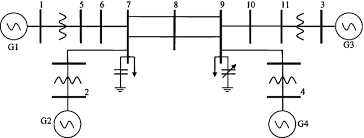
\includegraphics[width=0.5\textwidth]{pictures/kundurgrid.png}
    \caption{Kundur grid scheme. \cite{grids:kundur}}
    \label{fig:kundur2}
\end{figure}

This grid contains several devices including synchronous generators. To test this approach we define a new generator model called "GENROU bimode". This model has two different operating states that differ in the value of the parameter $M$ (the inertia of the rotor). The operating condition depends on $\omega$ the angular velocity of the generator's rotor. The angular velocity of the generator is the local measurement that the agent is adapting it's reacting to. We could imagine however an agent reacting to other measurements. Additionally, the derivative of $\omega$ depends on $M$ which will make the difference in the operating point very visible. Here is a summary of the simulation parameters and their interactions:\\

\begin{table}[H]
    \centering
    \begin{tabular}{|l|l|l|}
    \hline
    Operating State & Operating Condition                              & Parameter $M$ value \\ \hline
    A               & $\omega \in [1 - \varepsilon, 1 + \varepsilon]$ & 12  \\ \hline
    B               & $\omega \notin [1 - \varepsilon, 1 + \varepsilon]$ & 120               \\ \hline
    \end{tabular}
    \caption{Bimodal generator operating state summary.}
\end{table}

\begin{equation}
    \dot{\omega} = \frac{f(x, y)}{M}
\end{equation}

In this specific case we substitute one of the initial generators by a bimode generator. What we expect to see is the generator's angular velocity $\omega$ having 2 distinct behaviors. We run a time domain simulation to confirm our hypothesis. The simulation is run for over 20 seconds. The result conform to our hypothesis. 

Additionally, we can clearly see 2 discontinuities in the derivative of $\omega$. First at $t=2s$ when the line fault is triggered and then at around $t=3s$ when $\omega$ goes above the admissible interval ($\omega \geq \omega_{max} = 1.003 p.u. $).   

\begin{figure}[h]  % [h] places the figure "here"
    \centering
    % Fit the PGF figure to the page width
    \resizebox{\linewidth}{!}{%% Creator: Matplotlib, PGF backend
%%
%% To include the figure in your LaTeX document, write
%%   \input{<filename>.pgf}
%%
%% Make sure the required packages are loaded in your preamble
%%   \usepackage{pgf}
%%
%% Also ensure that all the required font packages are loaded; for instance,
%% the lmodern package is sometimes necessary when using math font.
%%   \usepackage{lmodern}
%%
%% Figures using additional raster images can only be included by \input if
%% they are in the same directory as the main LaTeX file. For loading figures
%% from other directories you can use the `import` package
%%   \usepackage{import}
%%
%% and then include the figures with
%%   \import{<path to file>}{<filename>.pgf}
%%
%% Matplotlib used the following preamble
%%   \def\mathdefault#1{#1}
%%   \everymath=\expandafter{\the\everymath\displaystyle}
%%   
%%   \ifdefined\pdftexversion\else  % non-pdftex case.
%%     \usepackage{fontspec}
%%     \setmainfont{DejaVuSerif.ttf}[Path=\detokenize{C:/Users/pablo/AppData/Local/Programs/Python/Python312/Lib/site-packages/matplotlib/mpl-data/fonts/ttf/}]
%%     \setsansfont{DejaVuSans.ttf}[Path=\detokenize{C:/Users/pablo/AppData/Local/Programs/Python/Python312/Lib/site-packages/matplotlib/mpl-data/fonts/ttf/}]
%%     \setmonofont{DejaVuSansMono.ttf}[Path=\detokenize{C:/Users/pablo/AppData/Local/Programs/Python/Python312/Lib/site-packages/matplotlib/mpl-data/fonts/ttf/}]
%%   \fi
%%   \makeatletter\@ifpackageloaded{underscore}{}{\usepackage[strings]{underscore}}\makeatother
%%
\begingroup%
\makeatletter%
\begin{pgfpicture}%
\pgfpathrectangle{\pgfpointorigin}{\pgfqpoint{6.400000in}{4.800000in}}%
\pgfusepath{use as bounding box, clip}%
\begin{pgfscope}%
\pgfsetbuttcap%
\pgfsetmiterjoin%
\definecolor{currentfill}{rgb}{1.000000,1.000000,1.000000}%
\pgfsetfillcolor{currentfill}%
\pgfsetlinewidth{0.000000pt}%
\definecolor{currentstroke}{rgb}{1.000000,1.000000,1.000000}%
\pgfsetstrokecolor{currentstroke}%
\pgfsetdash{}{0pt}%
\pgfpathmoveto{\pgfqpoint{0.000000in}{0.000000in}}%
\pgfpathlineto{\pgfqpoint{6.400000in}{0.000000in}}%
\pgfpathlineto{\pgfqpoint{6.400000in}{4.800000in}}%
\pgfpathlineto{\pgfqpoint{0.000000in}{4.800000in}}%
\pgfpathlineto{\pgfqpoint{0.000000in}{0.000000in}}%
\pgfpathclose%
\pgfusepath{fill}%
\end{pgfscope}%
\begin{pgfscope}%
\pgfsetbuttcap%
\pgfsetmiterjoin%
\definecolor{currentfill}{rgb}{1.000000,1.000000,1.000000}%
\pgfsetfillcolor{currentfill}%
\pgfsetlinewidth{0.000000pt}%
\definecolor{currentstroke}{rgb}{0.000000,0.000000,0.000000}%
\pgfsetstrokecolor{currentstroke}%
\pgfsetstrokeopacity{0.000000}%
\pgfsetdash{}{0pt}%
\pgfpathmoveto{\pgfqpoint{0.800000in}{0.528000in}}%
\pgfpathlineto{\pgfqpoint{5.760000in}{0.528000in}}%
\pgfpathlineto{\pgfqpoint{5.760000in}{4.224000in}}%
\pgfpathlineto{\pgfqpoint{0.800000in}{4.224000in}}%
\pgfpathlineto{\pgfqpoint{0.800000in}{0.528000in}}%
\pgfpathclose%
\pgfusepath{fill}%
\end{pgfscope}%
}

    \caption{Time series of the distributed generator's frequency.}
    \label{fig:sample_figure2}
\end{figure}

\subsection{Method 2: Time Domain solver change}

Another method to implement the different operating points for every agent is to directly change the parameters of the agent if necessary during each discrete time step of the solving algorithm. The algorithm follows these steps: it first checks the operating conditions and then performs the necessary changes. In pseudo-code the algorithm looks as follows: 

\begin{algorithm}
    \caption{TDS COLMENA}
    \begin{algorithmic}[1]
    \State Initialize grid states $x$ to $x_0$ through Power Flow results.
    \State $t \gets 0$
    \While{$t \leq t_{end}$}
        \For{agent in the set of Agents}
            \If{Operating Condition A(agent) is respected at time $t$}
                \State $mdl.param\_M \gets mdl.param\_M\_a$
            \Else 
                \State $mdl.param\_M  \gets mdl.param\_M\_b$
            \EndIf
        \EndFor
        \State Perform Trapezoid Step 
        \State Compute $x_{t+1}, y_{t+1}$
        \State $t \gets t + h$
    \EndWhile
    \State Finalize the result
    \end{algorithmic}
\end{algorithm}

In this case, the implementation is more flexible and we can imagine different changes or operating conditions that can be checked during each time step. However, the constraint of only basing the decisions on the context depends on how you check the condition and not directly on the model definition as before. 

\subsubsection{Case Study 2}

For this case study, we consider the 14 bus grid IEEE-14 \cite{grids:ieee14}. We consider a unique distributed generator which control the active and reactive power being injected to the grid. Here the agent with the role of the generator will have two operating points: one where he has an active power reference of $P_0$ and another with $-P_0$. The generator will change its operating state at $t=10s$. This is represented by the change in the parameter $\gamma_p$ from $0.1$ to $-0.1$. The simulation runs for 20s.\\ 
\begin{table}[H]
    \centering
    \begin{tabular}{|l|l|l|}
    \hline
    Operating State & Operating Condition  & Parameter $gamma_p$ value \\ \hline
    A               & $t \leq 10$ & 0.1  \\ \hline
    B               & $t \geq 10$ & -0.1  \\ \hline
    \end{tabular}
    \caption{Distributed generator state summary.}
\end{table}

As expected, we observe the change in operating time in the agent at $t =10s$. The change in frequency is what we expect from the change in power output. We also note that the initial frequency was of $60 Hz$ which is the standard in the USA instead of the $50 Hz$ that are used in Europe.

\begin{figure}[H]  % [h] places the figure "here"
    \centering
    % Fit the PGF figure to the page width
    \resizebox{\linewidth}{!}{%% Creator: Matplotlib, PGF backend
%%
%% To include the figure in your LaTeX document, write
%%   \input{<filename>.pgf}
%%
%% Make sure the required packages are loaded in your preamble
%%   \usepackage{pgf}
%%
%% Also ensure that all the required font packages are loaded; for instance,
%% the lmodern package is sometimes necessary when using math font.
%%   \usepackage{lmodern}
%%
%% Figures using additional raster images can only be included by \input if
%% they are in the same directory as the main LaTeX file. For loading figures
%% from other directories you can use the `import` package
%%   \usepackage{import}
%%
%% and then include the figures with
%%   \import{<path to file>}{<filename>.pgf}
%%
%% Matplotlib used the following preamble
%%   \def\mathdefault#1{#1}
%%   \everymath=\expandafter{\the\everymath\displaystyle}
%%   
%%   \usepackage{fontspec}
%%   \setmainfont{DejaVuSerif.ttf}[Path=\detokenize{C:/Users/Usuario/AppData/Local/Programs/Python/Python312/Lib/site-packages/matplotlib/mpl-data/fonts/ttf/}]
%%   \setsansfont{DejaVuSans.ttf}[Path=\detokenize{C:/Users/Usuario/AppData/Local/Programs/Python/Python312/Lib/site-packages/matplotlib/mpl-data/fonts/ttf/}]
%%   \setmonofont{DejaVuSansMono.ttf}[Path=\detokenize{C:/Users/Usuario/AppData/Local/Programs/Python/Python312/Lib/site-packages/matplotlib/mpl-data/fonts/ttf/}]
%%   \makeatletter\@ifpackageloaded{underscore}{}{\usepackage[strings]{underscore}}\makeatother
%%
\begingroup%
\makeatletter%
\begin{pgfpicture}%
\pgfpathrectangle{\pgfpointorigin}{\pgfqpoint{6.400000in}{4.800000in}}%
\pgfusepath{use as bounding box, clip}%
\begin{pgfscope}%
\pgfsetbuttcap%
\pgfsetmiterjoin%
\definecolor{currentfill}{rgb}{1.000000,1.000000,1.000000}%
\pgfsetfillcolor{currentfill}%
\pgfsetlinewidth{0.000000pt}%
\definecolor{currentstroke}{rgb}{1.000000,1.000000,1.000000}%
\pgfsetstrokecolor{currentstroke}%
\pgfsetdash{}{0pt}%
\pgfpathmoveto{\pgfqpoint{0.000000in}{0.000000in}}%
\pgfpathlineto{\pgfqpoint{6.400000in}{0.000000in}}%
\pgfpathlineto{\pgfqpoint{6.400000in}{4.800000in}}%
\pgfpathlineto{\pgfqpoint{0.000000in}{4.800000in}}%
\pgfpathlineto{\pgfqpoint{0.000000in}{0.000000in}}%
\pgfpathclose%
\pgfusepath{fill}%
\end{pgfscope}%
\begin{pgfscope}%
\pgfsetbuttcap%
\pgfsetmiterjoin%
\definecolor{currentfill}{rgb}{1.000000,1.000000,1.000000}%
\pgfsetfillcolor{currentfill}%
\pgfsetlinewidth{0.000000pt}%
\definecolor{currentstroke}{rgb}{0.000000,0.000000,0.000000}%
\pgfsetstrokecolor{currentstroke}%
\pgfsetstrokeopacity{0.000000}%
\pgfsetdash{}{0pt}%
\pgfpathmoveto{\pgfqpoint{0.800000in}{0.528000in}}%
\pgfpathlineto{\pgfqpoint{5.760000in}{0.528000in}}%
\pgfpathlineto{\pgfqpoint{5.760000in}{4.224000in}}%
\pgfpathlineto{\pgfqpoint{0.800000in}{4.224000in}}%
\pgfpathlineto{\pgfqpoint{0.800000in}{0.528000in}}%
\pgfpathclose%
\pgfusepath{fill}%
\end{pgfscope}%
\begin{pgfscope}%
\pgfsetbuttcap%
\pgfsetroundjoin%
\definecolor{currentfill}{rgb}{0.000000,0.000000,0.000000}%
\pgfsetfillcolor{currentfill}%
\pgfsetlinewidth{0.803000pt}%
\definecolor{currentstroke}{rgb}{0.000000,0.000000,0.000000}%
\pgfsetstrokecolor{currentstroke}%
\pgfsetdash{}{0pt}%
\pgfsys@defobject{currentmarker}{\pgfqpoint{0.000000in}{-0.048611in}}{\pgfqpoint{0.000000in}{0.000000in}}{%
\pgfpathmoveto{\pgfqpoint{0.000000in}{0.000000in}}%
\pgfpathlineto{\pgfqpoint{0.000000in}{-0.048611in}}%
\pgfusepath{stroke,fill}%
}%
\begin{pgfscope}%
\pgfsys@transformshift{0.800000in}{0.528000in}%
\pgfsys@useobject{currentmarker}{}%
\end{pgfscope}%
\end{pgfscope}%
\begin{pgfscope}%
\definecolor{textcolor}{rgb}{0.000000,0.000000,0.000000}%
\pgfsetstrokecolor{textcolor}%
\pgfsetfillcolor{textcolor}%
\pgftext[x=0.800000in,y=0.430778in,,top]{\color{textcolor}{\rmfamily\fontsize{12.000000}{14.400000}\selectfont\catcode`\^=\active\def^{\ifmmode\sp\else\^{}\fi}\catcode`\%=\active\def%{\%}$\mathdefault{0.0}$}}%
\end{pgfscope}%
\begin{pgfscope}%
\pgfsetbuttcap%
\pgfsetroundjoin%
\definecolor{currentfill}{rgb}{0.000000,0.000000,0.000000}%
\pgfsetfillcolor{currentfill}%
\pgfsetlinewidth{0.803000pt}%
\definecolor{currentstroke}{rgb}{0.000000,0.000000,0.000000}%
\pgfsetstrokecolor{currentstroke}%
\pgfsetdash{}{0pt}%
\pgfsys@defobject{currentmarker}{\pgfqpoint{0.000000in}{-0.048611in}}{\pgfqpoint{0.000000in}{0.000000in}}{%
\pgfpathmoveto{\pgfqpoint{0.000000in}{0.000000in}}%
\pgfpathlineto{\pgfqpoint{0.000000in}{-0.048611in}}%
\pgfusepath{stroke,fill}%
}%
\begin{pgfscope}%
\pgfsys@transformshift{1.420000in}{0.528000in}%
\pgfsys@useobject{currentmarker}{}%
\end{pgfscope}%
\end{pgfscope}%
\begin{pgfscope}%
\definecolor{textcolor}{rgb}{0.000000,0.000000,0.000000}%
\pgfsetstrokecolor{textcolor}%
\pgfsetfillcolor{textcolor}%
\pgftext[x=1.420000in,y=0.430778in,,top]{\color{textcolor}{\rmfamily\fontsize{12.000000}{14.400000}\selectfont\catcode`\^=\active\def^{\ifmmode\sp\else\^{}\fi}\catcode`\%=\active\def%{\%}$\mathdefault{2.5}$}}%
\end{pgfscope}%
\begin{pgfscope}%
\pgfsetbuttcap%
\pgfsetroundjoin%
\definecolor{currentfill}{rgb}{0.000000,0.000000,0.000000}%
\pgfsetfillcolor{currentfill}%
\pgfsetlinewidth{0.803000pt}%
\definecolor{currentstroke}{rgb}{0.000000,0.000000,0.000000}%
\pgfsetstrokecolor{currentstroke}%
\pgfsetdash{}{0pt}%
\pgfsys@defobject{currentmarker}{\pgfqpoint{0.000000in}{-0.048611in}}{\pgfqpoint{0.000000in}{0.000000in}}{%
\pgfpathmoveto{\pgfqpoint{0.000000in}{0.000000in}}%
\pgfpathlineto{\pgfqpoint{0.000000in}{-0.048611in}}%
\pgfusepath{stroke,fill}%
}%
\begin{pgfscope}%
\pgfsys@transformshift{2.040000in}{0.528000in}%
\pgfsys@useobject{currentmarker}{}%
\end{pgfscope}%
\end{pgfscope}%
\begin{pgfscope}%
\definecolor{textcolor}{rgb}{0.000000,0.000000,0.000000}%
\pgfsetstrokecolor{textcolor}%
\pgfsetfillcolor{textcolor}%
\pgftext[x=2.040000in,y=0.430778in,,top]{\color{textcolor}{\rmfamily\fontsize{12.000000}{14.400000}\selectfont\catcode`\^=\active\def^{\ifmmode\sp\else\^{}\fi}\catcode`\%=\active\def%{\%}$\mathdefault{5.0}$}}%
\end{pgfscope}%
\begin{pgfscope}%
\pgfsetbuttcap%
\pgfsetroundjoin%
\definecolor{currentfill}{rgb}{0.000000,0.000000,0.000000}%
\pgfsetfillcolor{currentfill}%
\pgfsetlinewidth{0.803000pt}%
\definecolor{currentstroke}{rgb}{0.000000,0.000000,0.000000}%
\pgfsetstrokecolor{currentstroke}%
\pgfsetdash{}{0pt}%
\pgfsys@defobject{currentmarker}{\pgfqpoint{0.000000in}{-0.048611in}}{\pgfqpoint{0.000000in}{0.000000in}}{%
\pgfpathmoveto{\pgfqpoint{0.000000in}{0.000000in}}%
\pgfpathlineto{\pgfqpoint{0.000000in}{-0.048611in}}%
\pgfusepath{stroke,fill}%
}%
\begin{pgfscope}%
\pgfsys@transformshift{2.660000in}{0.528000in}%
\pgfsys@useobject{currentmarker}{}%
\end{pgfscope}%
\end{pgfscope}%
\begin{pgfscope}%
\definecolor{textcolor}{rgb}{0.000000,0.000000,0.000000}%
\pgfsetstrokecolor{textcolor}%
\pgfsetfillcolor{textcolor}%
\pgftext[x=2.660000in,y=0.430778in,,top]{\color{textcolor}{\rmfamily\fontsize{12.000000}{14.400000}\selectfont\catcode`\^=\active\def^{\ifmmode\sp\else\^{}\fi}\catcode`\%=\active\def%{\%}$\mathdefault{7.5}$}}%
\end{pgfscope}%
\begin{pgfscope}%
\pgfsetbuttcap%
\pgfsetroundjoin%
\definecolor{currentfill}{rgb}{0.000000,0.000000,0.000000}%
\pgfsetfillcolor{currentfill}%
\pgfsetlinewidth{0.803000pt}%
\definecolor{currentstroke}{rgb}{0.000000,0.000000,0.000000}%
\pgfsetstrokecolor{currentstroke}%
\pgfsetdash{}{0pt}%
\pgfsys@defobject{currentmarker}{\pgfqpoint{0.000000in}{-0.048611in}}{\pgfqpoint{0.000000in}{0.000000in}}{%
\pgfpathmoveto{\pgfqpoint{0.000000in}{0.000000in}}%
\pgfpathlineto{\pgfqpoint{0.000000in}{-0.048611in}}%
\pgfusepath{stroke,fill}%
}%
\begin{pgfscope}%
\pgfsys@transformshift{3.280000in}{0.528000in}%
\pgfsys@useobject{currentmarker}{}%
\end{pgfscope}%
\end{pgfscope}%
\begin{pgfscope}%
\definecolor{textcolor}{rgb}{0.000000,0.000000,0.000000}%
\pgfsetstrokecolor{textcolor}%
\pgfsetfillcolor{textcolor}%
\pgftext[x=3.280000in,y=0.430778in,,top]{\color{textcolor}{\rmfamily\fontsize{12.000000}{14.400000}\selectfont\catcode`\^=\active\def^{\ifmmode\sp\else\^{}\fi}\catcode`\%=\active\def%{\%}$\mathdefault{10.0}$}}%
\end{pgfscope}%
\begin{pgfscope}%
\pgfsetbuttcap%
\pgfsetroundjoin%
\definecolor{currentfill}{rgb}{0.000000,0.000000,0.000000}%
\pgfsetfillcolor{currentfill}%
\pgfsetlinewidth{0.803000pt}%
\definecolor{currentstroke}{rgb}{0.000000,0.000000,0.000000}%
\pgfsetstrokecolor{currentstroke}%
\pgfsetdash{}{0pt}%
\pgfsys@defobject{currentmarker}{\pgfqpoint{0.000000in}{-0.048611in}}{\pgfqpoint{0.000000in}{0.000000in}}{%
\pgfpathmoveto{\pgfqpoint{0.000000in}{0.000000in}}%
\pgfpathlineto{\pgfqpoint{0.000000in}{-0.048611in}}%
\pgfusepath{stroke,fill}%
}%
\begin{pgfscope}%
\pgfsys@transformshift{3.900000in}{0.528000in}%
\pgfsys@useobject{currentmarker}{}%
\end{pgfscope}%
\end{pgfscope}%
\begin{pgfscope}%
\definecolor{textcolor}{rgb}{0.000000,0.000000,0.000000}%
\pgfsetstrokecolor{textcolor}%
\pgfsetfillcolor{textcolor}%
\pgftext[x=3.900000in,y=0.430778in,,top]{\color{textcolor}{\rmfamily\fontsize{12.000000}{14.400000}\selectfont\catcode`\^=\active\def^{\ifmmode\sp\else\^{}\fi}\catcode`\%=\active\def%{\%}$\mathdefault{12.5}$}}%
\end{pgfscope}%
\begin{pgfscope}%
\pgfsetbuttcap%
\pgfsetroundjoin%
\definecolor{currentfill}{rgb}{0.000000,0.000000,0.000000}%
\pgfsetfillcolor{currentfill}%
\pgfsetlinewidth{0.803000pt}%
\definecolor{currentstroke}{rgb}{0.000000,0.000000,0.000000}%
\pgfsetstrokecolor{currentstroke}%
\pgfsetdash{}{0pt}%
\pgfsys@defobject{currentmarker}{\pgfqpoint{0.000000in}{-0.048611in}}{\pgfqpoint{0.000000in}{0.000000in}}{%
\pgfpathmoveto{\pgfqpoint{0.000000in}{0.000000in}}%
\pgfpathlineto{\pgfqpoint{0.000000in}{-0.048611in}}%
\pgfusepath{stroke,fill}%
}%
\begin{pgfscope}%
\pgfsys@transformshift{4.520000in}{0.528000in}%
\pgfsys@useobject{currentmarker}{}%
\end{pgfscope}%
\end{pgfscope}%
\begin{pgfscope}%
\definecolor{textcolor}{rgb}{0.000000,0.000000,0.000000}%
\pgfsetstrokecolor{textcolor}%
\pgfsetfillcolor{textcolor}%
\pgftext[x=4.520000in,y=0.430778in,,top]{\color{textcolor}{\rmfamily\fontsize{12.000000}{14.400000}\selectfont\catcode`\^=\active\def^{\ifmmode\sp\else\^{}\fi}\catcode`\%=\active\def%{\%}$\mathdefault{15.0}$}}%
\end{pgfscope}%
\begin{pgfscope}%
\pgfsetbuttcap%
\pgfsetroundjoin%
\definecolor{currentfill}{rgb}{0.000000,0.000000,0.000000}%
\pgfsetfillcolor{currentfill}%
\pgfsetlinewidth{0.803000pt}%
\definecolor{currentstroke}{rgb}{0.000000,0.000000,0.000000}%
\pgfsetstrokecolor{currentstroke}%
\pgfsetdash{}{0pt}%
\pgfsys@defobject{currentmarker}{\pgfqpoint{0.000000in}{-0.048611in}}{\pgfqpoint{0.000000in}{0.000000in}}{%
\pgfpathmoveto{\pgfqpoint{0.000000in}{0.000000in}}%
\pgfpathlineto{\pgfqpoint{0.000000in}{-0.048611in}}%
\pgfusepath{stroke,fill}%
}%
\begin{pgfscope}%
\pgfsys@transformshift{5.140000in}{0.528000in}%
\pgfsys@useobject{currentmarker}{}%
\end{pgfscope}%
\end{pgfscope}%
\begin{pgfscope}%
\definecolor{textcolor}{rgb}{0.000000,0.000000,0.000000}%
\pgfsetstrokecolor{textcolor}%
\pgfsetfillcolor{textcolor}%
\pgftext[x=5.140000in,y=0.430778in,,top]{\color{textcolor}{\rmfamily\fontsize{12.000000}{14.400000}\selectfont\catcode`\^=\active\def^{\ifmmode\sp\else\^{}\fi}\catcode`\%=\active\def%{\%}$\mathdefault{17.5}$}}%
\end{pgfscope}%
\begin{pgfscope}%
\pgfsetbuttcap%
\pgfsetroundjoin%
\definecolor{currentfill}{rgb}{0.000000,0.000000,0.000000}%
\pgfsetfillcolor{currentfill}%
\pgfsetlinewidth{0.803000pt}%
\definecolor{currentstroke}{rgb}{0.000000,0.000000,0.000000}%
\pgfsetstrokecolor{currentstroke}%
\pgfsetdash{}{0pt}%
\pgfsys@defobject{currentmarker}{\pgfqpoint{0.000000in}{-0.048611in}}{\pgfqpoint{0.000000in}{0.000000in}}{%
\pgfpathmoveto{\pgfqpoint{0.000000in}{0.000000in}}%
\pgfpathlineto{\pgfqpoint{0.000000in}{-0.048611in}}%
\pgfusepath{stroke,fill}%
}%
\begin{pgfscope}%
\pgfsys@transformshift{5.760000in}{0.528000in}%
\pgfsys@useobject{currentmarker}{}%
\end{pgfscope}%
\end{pgfscope}%
\begin{pgfscope}%
\definecolor{textcolor}{rgb}{0.000000,0.000000,0.000000}%
\pgfsetstrokecolor{textcolor}%
\pgfsetfillcolor{textcolor}%
\pgftext[x=5.760000in,y=0.430778in,,top]{\color{textcolor}{\rmfamily\fontsize{12.000000}{14.400000}\selectfont\catcode`\^=\active\def^{\ifmmode\sp\else\^{}\fi}\catcode`\%=\active\def%{\%}$\mathdefault{20.0}$}}%
\end{pgfscope}%
\begin{pgfscope}%
\definecolor{textcolor}{rgb}{0.000000,0.000000,0.000000}%
\pgfsetstrokecolor{textcolor}%
\pgfsetfillcolor{textcolor}%
\pgftext[x=3.280000in,y=0.213927in,,top]{\color{textcolor}{\rmfamily\fontsize{12.000000}{14.400000}\selectfont\catcode`\^=\active\def^{\ifmmode\sp\else\^{}\fi}\catcode`\%=\active\def%{\%}Time [s]}}%
\end{pgfscope}%
\begin{pgfscope}%
\pgfsetbuttcap%
\pgfsetroundjoin%
\definecolor{currentfill}{rgb}{0.000000,0.000000,0.000000}%
\pgfsetfillcolor{currentfill}%
\pgfsetlinewidth{0.803000pt}%
\definecolor{currentstroke}{rgb}{0.000000,0.000000,0.000000}%
\pgfsetstrokecolor{currentstroke}%
\pgfsetdash{}{0pt}%
\pgfsys@defobject{currentmarker}{\pgfqpoint{-0.048611in}{0.000000in}}{\pgfqpoint{-0.000000in}{0.000000in}}{%
\pgfpathmoveto{\pgfqpoint{-0.000000in}{0.000000in}}%
\pgfpathlineto{\pgfqpoint{-0.048611in}{0.000000in}}%
\pgfusepath{stroke,fill}%
}%
\begin{pgfscope}%
\pgfsys@transformshift{0.800000in}{0.647536in}%
\pgfsys@useobject{currentmarker}{}%
\end{pgfscope}%
\end{pgfscope}%
\begin{pgfscope}%
\definecolor{textcolor}{rgb}{0.000000,0.000000,0.000000}%
\pgfsetstrokecolor{textcolor}%
\pgfsetfillcolor{textcolor}%
\pgftext[x=0.167868in, y=0.584223in, left, base]{\color{textcolor}{\rmfamily\fontsize{12.000000}{14.400000}\selectfont\catcode`\^=\active\def^{\ifmmode\sp\else\^{}\fi}\catcode`\%=\active\def%{\%}$\mathdefault{59.9970}$}}%
\end{pgfscope}%
\begin{pgfscope}%
\pgfsetbuttcap%
\pgfsetroundjoin%
\definecolor{currentfill}{rgb}{0.000000,0.000000,0.000000}%
\pgfsetfillcolor{currentfill}%
\pgfsetlinewidth{0.803000pt}%
\definecolor{currentstroke}{rgb}{0.000000,0.000000,0.000000}%
\pgfsetstrokecolor{currentstroke}%
\pgfsetdash{}{0pt}%
\pgfsys@defobject{currentmarker}{\pgfqpoint{-0.048611in}{0.000000in}}{\pgfqpoint{-0.000000in}{0.000000in}}{%
\pgfpathmoveto{\pgfqpoint{-0.000000in}{0.000000in}}%
\pgfpathlineto{\pgfqpoint{-0.048611in}{0.000000in}}%
\pgfusepath{stroke,fill}%
}%
\begin{pgfscope}%
\pgfsys@transformshift{0.800000in}{1.215614in}%
\pgfsys@useobject{currentmarker}{}%
\end{pgfscope}%
\end{pgfscope}%
\begin{pgfscope}%
\definecolor{textcolor}{rgb}{0.000000,0.000000,0.000000}%
\pgfsetstrokecolor{textcolor}%
\pgfsetfillcolor{textcolor}%
\pgftext[x=0.167868in, y=1.152300in, left, base]{\color{textcolor}{\rmfamily\fontsize{12.000000}{14.400000}\selectfont\catcode`\^=\active\def^{\ifmmode\sp\else\^{}\fi}\catcode`\%=\active\def%{\%}$\mathdefault{59.9975}$}}%
\end{pgfscope}%
\begin{pgfscope}%
\pgfsetbuttcap%
\pgfsetroundjoin%
\definecolor{currentfill}{rgb}{0.000000,0.000000,0.000000}%
\pgfsetfillcolor{currentfill}%
\pgfsetlinewidth{0.803000pt}%
\definecolor{currentstroke}{rgb}{0.000000,0.000000,0.000000}%
\pgfsetstrokecolor{currentstroke}%
\pgfsetdash{}{0pt}%
\pgfsys@defobject{currentmarker}{\pgfqpoint{-0.048611in}{0.000000in}}{\pgfqpoint{-0.000000in}{0.000000in}}{%
\pgfpathmoveto{\pgfqpoint{-0.000000in}{0.000000in}}%
\pgfpathlineto{\pgfqpoint{-0.048611in}{0.000000in}}%
\pgfusepath{stroke,fill}%
}%
\begin{pgfscope}%
\pgfsys@transformshift{0.800000in}{1.783691in}%
\pgfsys@useobject{currentmarker}{}%
\end{pgfscope}%
\end{pgfscope}%
\begin{pgfscope}%
\definecolor{textcolor}{rgb}{0.000000,0.000000,0.000000}%
\pgfsetstrokecolor{textcolor}%
\pgfsetfillcolor{textcolor}%
\pgftext[x=0.167868in, y=1.720377in, left, base]{\color{textcolor}{\rmfamily\fontsize{12.000000}{14.400000}\selectfont\catcode`\^=\active\def^{\ifmmode\sp\else\^{}\fi}\catcode`\%=\active\def%{\%}$\mathdefault{59.9980}$}}%
\end{pgfscope}%
\begin{pgfscope}%
\pgfsetbuttcap%
\pgfsetroundjoin%
\definecolor{currentfill}{rgb}{0.000000,0.000000,0.000000}%
\pgfsetfillcolor{currentfill}%
\pgfsetlinewidth{0.803000pt}%
\definecolor{currentstroke}{rgb}{0.000000,0.000000,0.000000}%
\pgfsetstrokecolor{currentstroke}%
\pgfsetdash{}{0pt}%
\pgfsys@defobject{currentmarker}{\pgfqpoint{-0.048611in}{0.000000in}}{\pgfqpoint{-0.000000in}{0.000000in}}{%
\pgfpathmoveto{\pgfqpoint{-0.000000in}{0.000000in}}%
\pgfpathlineto{\pgfqpoint{-0.048611in}{0.000000in}}%
\pgfusepath{stroke,fill}%
}%
\begin{pgfscope}%
\pgfsys@transformshift{0.800000in}{2.351768in}%
\pgfsys@useobject{currentmarker}{}%
\end{pgfscope}%
\end{pgfscope}%
\begin{pgfscope}%
\definecolor{textcolor}{rgb}{0.000000,0.000000,0.000000}%
\pgfsetstrokecolor{textcolor}%
\pgfsetfillcolor{textcolor}%
\pgftext[x=0.167868in, y=2.288454in, left, base]{\color{textcolor}{\rmfamily\fontsize{12.000000}{14.400000}\selectfont\catcode`\^=\active\def^{\ifmmode\sp\else\^{}\fi}\catcode`\%=\active\def%{\%}$\mathdefault{59.9985}$}}%
\end{pgfscope}%
\begin{pgfscope}%
\pgfsetbuttcap%
\pgfsetroundjoin%
\definecolor{currentfill}{rgb}{0.000000,0.000000,0.000000}%
\pgfsetfillcolor{currentfill}%
\pgfsetlinewidth{0.803000pt}%
\definecolor{currentstroke}{rgb}{0.000000,0.000000,0.000000}%
\pgfsetstrokecolor{currentstroke}%
\pgfsetdash{}{0pt}%
\pgfsys@defobject{currentmarker}{\pgfqpoint{-0.048611in}{0.000000in}}{\pgfqpoint{-0.000000in}{0.000000in}}{%
\pgfpathmoveto{\pgfqpoint{-0.000000in}{0.000000in}}%
\pgfpathlineto{\pgfqpoint{-0.048611in}{0.000000in}}%
\pgfusepath{stroke,fill}%
}%
\begin{pgfscope}%
\pgfsys@transformshift{0.800000in}{2.919845in}%
\pgfsys@useobject{currentmarker}{}%
\end{pgfscope}%
\end{pgfscope}%
\begin{pgfscope}%
\definecolor{textcolor}{rgb}{0.000000,0.000000,0.000000}%
\pgfsetstrokecolor{textcolor}%
\pgfsetfillcolor{textcolor}%
\pgftext[x=0.167868in, y=2.856532in, left, base]{\color{textcolor}{\rmfamily\fontsize{12.000000}{14.400000}\selectfont\catcode`\^=\active\def^{\ifmmode\sp\else\^{}\fi}\catcode`\%=\active\def%{\%}$\mathdefault{59.9990}$}}%
\end{pgfscope}%
\begin{pgfscope}%
\pgfsetbuttcap%
\pgfsetroundjoin%
\definecolor{currentfill}{rgb}{0.000000,0.000000,0.000000}%
\pgfsetfillcolor{currentfill}%
\pgfsetlinewidth{0.803000pt}%
\definecolor{currentstroke}{rgb}{0.000000,0.000000,0.000000}%
\pgfsetstrokecolor{currentstroke}%
\pgfsetdash{}{0pt}%
\pgfsys@defobject{currentmarker}{\pgfqpoint{-0.048611in}{0.000000in}}{\pgfqpoint{-0.000000in}{0.000000in}}{%
\pgfpathmoveto{\pgfqpoint{-0.000000in}{0.000000in}}%
\pgfpathlineto{\pgfqpoint{-0.048611in}{0.000000in}}%
\pgfusepath{stroke,fill}%
}%
\begin{pgfscope}%
\pgfsys@transformshift{0.800000in}{3.487923in}%
\pgfsys@useobject{currentmarker}{}%
\end{pgfscope}%
\end{pgfscope}%
\begin{pgfscope}%
\definecolor{textcolor}{rgb}{0.000000,0.000000,0.000000}%
\pgfsetstrokecolor{textcolor}%
\pgfsetfillcolor{textcolor}%
\pgftext[x=0.167868in, y=3.424609in, left, base]{\color{textcolor}{\rmfamily\fontsize{12.000000}{14.400000}\selectfont\catcode`\^=\active\def^{\ifmmode\sp\else\^{}\fi}\catcode`\%=\active\def%{\%}$\mathdefault{59.9995}$}}%
\end{pgfscope}%
\begin{pgfscope}%
\pgfsetbuttcap%
\pgfsetroundjoin%
\definecolor{currentfill}{rgb}{0.000000,0.000000,0.000000}%
\pgfsetfillcolor{currentfill}%
\pgfsetlinewidth{0.803000pt}%
\definecolor{currentstroke}{rgb}{0.000000,0.000000,0.000000}%
\pgfsetstrokecolor{currentstroke}%
\pgfsetdash{}{0pt}%
\pgfsys@defobject{currentmarker}{\pgfqpoint{-0.048611in}{0.000000in}}{\pgfqpoint{-0.000000in}{0.000000in}}{%
\pgfpathmoveto{\pgfqpoint{-0.000000in}{0.000000in}}%
\pgfpathlineto{\pgfqpoint{-0.048611in}{0.000000in}}%
\pgfusepath{stroke,fill}%
}%
\begin{pgfscope}%
\pgfsys@transformshift{0.800000in}{4.056000in}%
\pgfsys@useobject{currentmarker}{}%
\end{pgfscope}%
\end{pgfscope}%
\begin{pgfscope}%
\definecolor{textcolor}{rgb}{0.000000,0.000000,0.000000}%
\pgfsetstrokecolor{textcolor}%
\pgfsetfillcolor{textcolor}%
\pgftext[x=0.167868in, y=3.992686in, left, base]{\color{textcolor}{\rmfamily\fontsize{12.000000}{14.400000}\selectfont\catcode`\^=\active\def^{\ifmmode\sp\else\^{}\fi}\catcode`\%=\active\def%{\%}$\mathdefault{60.0000}$}}%
\end{pgfscope}%
\begin{pgfscope}%
\pgfpathrectangle{\pgfqpoint{0.800000in}{0.528000in}}{\pgfqpoint{4.960000in}{3.696000in}}%
\pgfusepath{clip}%
\pgfsetrectcap%
\pgfsetroundjoin%
\pgfsetlinewidth{1.003750pt}%
\definecolor{currentstroke}{rgb}{0.121569,0.466667,0.705882}%
\pgfsetstrokecolor{currentstroke}%
\pgfsetdash{}{0pt}%
\pgfpathmoveto{\pgfqpoint{0.800000in}{4.056000in}}%
\pgfpathlineto{\pgfqpoint{3.274238in}{4.056000in}}%
\pgfpathlineto{\pgfqpoint{3.282505in}{3.488196in}}%
\pgfpathlineto{\pgfqpoint{3.290771in}{2.615792in}}%
\pgfpathlineto{\pgfqpoint{3.299038in}{2.655251in}}%
\pgfpathlineto{\pgfqpoint{3.307305in}{3.064724in}}%
\pgfpathlineto{\pgfqpoint{3.315571in}{3.105124in}}%
\pgfpathlineto{\pgfqpoint{3.323838in}{3.045701in}}%
\pgfpathlineto{\pgfqpoint{3.332105in}{2.963644in}}%
\pgfpathlineto{\pgfqpoint{3.348638in}{2.738917in}}%
\pgfpathlineto{\pgfqpoint{3.389971in}{2.136182in}}%
\pgfpathlineto{\pgfqpoint{3.406505in}{1.920216in}}%
\pgfpathlineto{\pgfqpoint{3.423038in}{1.724561in}}%
\pgfpathlineto{\pgfqpoint{3.439571in}{1.549775in}}%
\pgfpathlineto{\pgfqpoint{3.456105in}{1.395597in}}%
\pgfpathlineto{\pgfqpoint{3.472638in}{1.261316in}}%
\pgfpathlineto{\pgfqpoint{3.489171in}{1.145924in}}%
\pgfpathlineto{\pgfqpoint{3.505705in}{1.048166in}}%
\pgfpathlineto{\pgfqpoint{3.522238in}{0.966581in}}%
\pgfpathlineto{\pgfqpoint{3.538771in}{0.899542in}}%
\pgfpathlineto{\pgfqpoint{3.555305in}{0.845338in}}%
\pgfpathlineto{\pgfqpoint{3.571838in}{0.802253in}}%
\pgfpathlineto{\pgfqpoint{3.588371in}{0.768650in}}%
\pgfpathlineto{\pgfqpoint{3.604905in}{0.743044in}}%
\pgfpathlineto{\pgfqpoint{3.621438in}{0.724136in}}%
\pgfpathlineto{\pgfqpoint{3.637971in}{0.710824in}}%
\pgfpathlineto{\pgfqpoint{3.654505in}{0.702191in}}%
\pgfpathlineto{\pgfqpoint{3.671038in}{0.697469in}}%
\pgfpathlineto{\pgfqpoint{3.687571in}{0.696000in}}%
\pgfpathlineto{\pgfqpoint{3.704105in}{0.697205in}}%
\pgfpathlineto{\pgfqpoint{3.720638in}{0.700559in}}%
\pgfpathlineto{\pgfqpoint{3.745438in}{0.708574in}}%
\pgfpathlineto{\pgfqpoint{3.778505in}{0.722659in}}%
\pgfpathlineto{\pgfqpoint{3.919038in}{0.787003in}}%
\pgfpathlineto{\pgfqpoint{3.985171in}{0.813607in}}%
\pgfpathlineto{\pgfqpoint{4.043038in}{0.834323in}}%
\pgfpathlineto{\pgfqpoint{4.109171in}{0.855489in}}%
\pgfpathlineto{\pgfqpoint{4.795305in}{1.065014in}}%
\pgfpathlineto{\pgfqpoint{4.927571in}{1.102206in}}%
\pgfpathlineto{\pgfqpoint{5.051571in}{1.134692in}}%
\pgfpathlineto{\pgfqpoint{5.167305in}{1.162769in}}%
\pgfpathlineto{\pgfqpoint{5.283038in}{1.188638in}}%
\pgfpathlineto{\pgfqpoint{5.398771in}{1.212320in}}%
\pgfpathlineto{\pgfqpoint{5.522771in}{1.235343in}}%
\pgfpathlineto{\pgfqpoint{5.646771in}{1.256054in}}%
\pgfpathlineto{\pgfqpoint{5.760000in}{1.273073in}}%
\pgfpathlineto{\pgfqpoint{5.760000in}{1.273073in}}%
\pgfusepath{stroke}%
\end{pgfscope}%
\begin{pgfscope}%
\pgfsetrectcap%
\pgfsetmiterjoin%
\pgfsetlinewidth{0.803000pt}%
\definecolor{currentstroke}{rgb}{0.000000,0.000000,0.000000}%
\pgfsetstrokecolor{currentstroke}%
\pgfsetdash{}{0pt}%
\pgfpathmoveto{\pgfqpoint{0.800000in}{0.528000in}}%
\pgfpathlineto{\pgfqpoint{0.800000in}{4.224000in}}%
\pgfusepath{stroke}%
\end{pgfscope}%
\begin{pgfscope}%
\pgfsetrectcap%
\pgfsetmiterjoin%
\pgfsetlinewidth{0.803000pt}%
\definecolor{currentstroke}{rgb}{0.000000,0.000000,0.000000}%
\pgfsetstrokecolor{currentstroke}%
\pgfsetdash{}{0pt}%
\pgfpathmoveto{\pgfqpoint{5.760000in}{0.528000in}}%
\pgfpathlineto{\pgfqpoint{5.760000in}{4.224000in}}%
\pgfusepath{stroke}%
\end{pgfscope}%
\begin{pgfscope}%
\pgfsetrectcap%
\pgfsetmiterjoin%
\pgfsetlinewidth{0.803000pt}%
\definecolor{currentstroke}{rgb}{0.000000,0.000000,0.000000}%
\pgfsetstrokecolor{currentstroke}%
\pgfsetdash{}{0pt}%
\pgfpathmoveto{\pgfqpoint{0.800000in}{0.528000in}}%
\pgfpathlineto{\pgfqpoint{5.760000in}{0.528000in}}%
\pgfusepath{stroke}%
\end{pgfscope}%
\begin{pgfscope}%
\pgfsetrectcap%
\pgfsetmiterjoin%
\pgfsetlinewidth{0.803000pt}%
\definecolor{currentstroke}{rgb}{0.000000,0.000000,0.000000}%
\pgfsetstrokecolor{currentstroke}%
\pgfsetdash{}{0pt}%
\pgfpathmoveto{\pgfqpoint{0.800000in}{4.224000in}}%
\pgfpathlineto{\pgfqpoint{5.760000in}{4.224000in}}%
\pgfusepath{stroke}%
\end{pgfscope}%
\begin{pgfscope}%
\pgfsetrectcap%
\pgfsetroundjoin%
\pgfsetlinewidth{1.003750pt}%
\definecolor{currentstroke}{rgb}{0.121569,0.466667,0.705882}%
\pgfsetstrokecolor{currentstroke}%
\pgfsetdash{}{0pt}%
\pgfpathmoveto{\pgfqpoint{4.206642in}{4.005706in}}%
\pgfpathlineto{\pgfqpoint{4.373308in}{4.005706in}}%
\pgfpathlineto{\pgfqpoint{4.539975in}{4.005706in}}%
\pgfusepath{stroke}%
\end{pgfscope}%
\begin{pgfscope}%
\definecolor{textcolor}{rgb}{0.000000,0.000000,0.000000}%
\pgfsetstrokecolor{textcolor}%
\pgfsetfillcolor{textcolor}%
\pgftext[x=4.673308in,y=3.947372in,left,base]{\color{textcolor}{\rmfamily\fontsize{12.000000}{14.400000}\selectfont\catcode`\^=\active\def^{\ifmmode\sp\else\^{}\fi}\catcode`\%=\active\def%{\%}$f_{Hz}$ PVD1 1}}%
\end{pgfscope}%
\end{pgfpicture}%
\makeatother%
\endgroup%
}
% %% Creator: Matplotlib, PGF backend
%%
%% To include the figure in your LaTeX document, write
%%   \input{<filename>.pgf}
%%
%% Make sure the required packages are loaded in your preamble
%%   \usepackage{pgf}
%%
%% Also ensure that all the required font packages are loaded; for instance,
%% the lmodern package is sometimes necessary when using math font.
%%   \usepackage{lmodern}
%%
%% Figures using additional raster images can only be included by \input if
%% they are in the same directory as the main LaTeX file. For loading figures
%% from other directories you can use the `import` package
%%   \usepackage{import}
%%
%% and then include the figures with
%%   \import{<path to file>}{<filename>.pgf}
%%
%% Matplotlib used the following preamble
%%   \def\mathdefault#1{#1}
%%   \everymath=\expandafter{\the\everymath\displaystyle}
%%   
%%   \usepackage{fontspec}
%%   \setmainfont{DejaVuSerif.ttf}[Path=\detokenize{C:/Users/Usuario/AppData/Local/Programs/Python/Python312/Lib/site-packages/matplotlib/mpl-data/fonts/ttf/}]
%%   \setsansfont{DejaVuSans.ttf}[Path=\detokenize{C:/Users/Usuario/AppData/Local/Programs/Python/Python312/Lib/site-packages/matplotlib/mpl-data/fonts/ttf/}]
%%   \setmonofont{DejaVuSansMono.ttf}[Path=\detokenize{C:/Users/Usuario/AppData/Local/Programs/Python/Python312/Lib/site-packages/matplotlib/mpl-data/fonts/ttf/}]
%%   \makeatletter\@ifpackageloaded{underscore}{}{\usepackage[strings]{underscore}}\makeatother
%%
\begingroup%
\makeatletter%
\begin{pgfpicture}%
\pgfpathrectangle{\pgfpointorigin}{\pgfqpoint{6.400000in}{4.800000in}}%
\pgfusepath{use as bounding box, clip}%
\begin{pgfscope}%
\pgfsetbuttcap%
\pgfsetmiterjoin%
\definecolor{currentfill}{rgb}{1.000000,1.000000,1.000000}%
\pgfsetfillcolor{currentfill}%
\pgfsetlinewidth{0.000000pt}%
\definecolor{currentstroke}{rgb}{1.000000,1.000000,1.000000}%
\pgfsetstrokecolor{currentstroke}%
\pgfsetdash{}{0pt}%
\pgfpathmoveto{\pgfqpoint{0.000000in}{0.000000in}}%
\pgfpathlineto{\pgfqpoint{6.400000in}{0.000000in}}%
\pgfpathlineto{\pgfqpoint{6.400000in}{4.800000in}}%
\pgfpathlineto{\pgfqpoint{0.000000in}{4.800000in}}%
\pgfpathlineto{\pgfqpoint{0.000000in}{0.000000in}}%
\pgfpathclose%
\pgfusepath{fill}%
\end{pgfscope}%
\begin{pgfscope}%
\pgfsetbuttcap%
\pgfsetmiterjoin%
\definecolor{currentfill}{rgb}{1.000000,1.000000,1.000000}%
\pgfsetfillcolor{currentfill}%
\pgfsetlinewidth{0.000000pt}%
\definecolor{currentstroke}{rgb}{0.000000,0.000000,0.000000}%
\pgfsetstrokecolor{currentstroke}%
\pgfsetstrokeopacity{0.000000}%
\pgfsetdash{}{0pt}%
\pgfpathmoveto{\pgfqpoint{0.800000in}{0.528000in}}%
\pgfpathlineto{\pgfqpoint{5.760000in}{0.528000in}}%
\pgfpathlineto{\pgfqpoint{5.760000in}{4.224000in}}%
\pgfpathlineto{\pgfqpoint{0.800000in}{4.224000in}}%
\pgfpathlineto{\pgfqpoint{0.800000in}{0.528000in}}%
\pgfpathclose%
\pgfusepath{fill}%
\end{pgfscope}%
\begin{pgfscope}%
\pgfsetbuttcap%
\pgfsetroundjoin%
\definecolor{currentfill}{rgb}{0.000000,0.000000,0.000000}%
\pgfsetfillcolor{currentfill}%
\pgfsetlinewidth{0.803000pt}%
\definecolor{currentstroke}{rgb}{0.000000,0.000000,0.000000}%
\pgfsetstrokecolor{currentstroke}%
\pgfsetdash{}{0pt}%
\pgfsys@defobject{currentmarker}{\pgfqpoint{0.000000in}{-0.048611in}}{\pgfqpoint{0.000000in}{0.000000in}}{%
\pgfpathmoveto{\pgfqpoint{0.000000in}{0.000000in}}%
\pgfpathlineto{\pgfqpoint{0.000000in}{-0.048611in}}%
\pgfusepath{stroke,fill}%
}%
\begin{pgfscope}%
\pgfsys@transformshift{0.800000in}{0.528000in}%
\pgfsys@useobject{currentmarker}{}%
\end{pgfscope}%
\end{pgfscope}%
\begin{pgfscope}%
\definecolor{textcolor}{rgb}{0.000000,0.000000,0.000000}%
\pgfsetstrokecolor{textcolor}%
\pgfsetfillcolor{textcolor}%
\pgftext[x=0.800000in,y=0.430778in,,top]{\color{textcolor}{\rmfamily\fontsize{12.000000}{14.400000}\selectfont\catcode`\^=\active\def^{\ifmmode\sp\else\^{}\fi}\catcode`\%=\active\def%{\%}$\mathdefault{0.0}$}}%
\end{pgfscope}%
\begin{pgfscope}%
\pgfsetbuttcap%
\pgfsetroundjoin%
\definecolor{currentfill}{rgb}{0.000000,0.000000,0.000000}%
\pgfsetfillcolor{currentfill}%
\pgfsetlinewidth{0.803000pt}%
\definecolor{currentstroke}{rgb}{0.000000,0.000000,0.000000}%
\pgfsetstrokecolor{currentstroke}%
\pgfsetdash{}{0pt}%
\pgfsys@defobject{currentmarker}{\pgfqpoint{0.000000in}{-0.048611in}}{\pgfqpoint{0.000000in}{0.000000in}}{%
\pgfpathmoveto{\pgfqpoint{0.000000in}{0.000000in}}%
\pgfpathlineto{\pgfqpoint{0.000000in}{-0.048611in}}%
\pgfusepath{stroke,fill}%
}%
\begin{pgfscope}%
\pgfsys@transformshift{1.420000in}{0.528000in}%
\pgfsys@useobject{currentmarker}{}%
\end{pgfscope}%
\end{pgfscope}%
\begin{pgfscope}%
\definecolor{textcolor}{rgb}{0.000000,0.000000,0.000000}%
\pgfsetstrokecolor{textcolor}%
\pgfsetfillcolor{textcolor}%
\pgftext[x=1.420000in,y=0.430778in,,top]{\color{textcolor}{\rmfamily\fontsize{12.000000}{14.400000}\selectfont\catcode`\^=\active\def^{\ifmmode\sp\else\^{}\fi}\catcode`\%=\active\def%{\%}$\mathdefault{2.5}$}}%
\end{pgfscope}%
\begin{pgfscope}%
\pgfsetbuttcap%
\pgfsetroundjoin%
\definecolor{currentfill}{rgb}{0.000000,0.000000,0.000000}%
\pgfsetfillcolor{currentfill}%
\pgfsetlinewidth{0.803000pt}%
\definecolor{currentstroke}{rgb}{0.000000,0.000000,0.000000}%
\pgfsetstrokecolor{currentstroke}%
\pgfsetdash{}{0pt}%
\pgfsys@defobject{currentmarker}{\pgfqpoint{0.000000in}{-0.048611in}}{\pgfqpoint{0.000000in}{0.000000in}}{%
\pgfpathmoveto{\pgfqpoint{0.000000in}{0.000000in}}%
\pgfpathlineto{\pgfqpoint{0.000000in}{-0.048611in}}%
\pgfusepath{stroke,fill}%
}%
\begin{pgfscope}%
\pgfsys@transformshift{2.040000in}{0.528000in}%
\pgfsys@useobject{currentmarker}{}%
\end{pgfscope}%
\end{pgfscope}%
\begin{pgfscope}%
\definecolor{textcolor}{rgb}{0.000000,0.000000,0.000000}%
\pgfsetstrokecolor{textcolor}%
\pgfsetfillcolor{textcolor}%
\pgftext[x=2.040000in,y=0.430778in,,top]{\color{textcolor}{\rmfamily\fontsize{12.000000}{14.400000}\selectfont\catcode`\^=\active\def^{\ifmmode\sp\else\^{}\fi}\catcode`\%=\active\def%{\%}$\mathdefault{5.0}$}}%
\end{pgfscope}%
\begin{pgfscope}%
\pgfsetbuttcap%
\pgfsetroundjoin%
\definecolor{currentfill}{rgb}{0.000000,0.000000,0.000000}%
\pgfsetfillcolor{currentfill}%
\pgfsetlinewidth{0.803000pt}%
\definecolor{currentstroke}{rgb}{0.000000,0.000000,0.000000}%
\pgfsetstrokecolor{currentstroke}%
\pgfsetdash{}{0pt}%
\pgfsys@defobject{currentmarker}{\pgfqpoint{0.000000in}{-0.048611in}}{\pgfqpoint{0.000000in}{0.000000in}}{%
\pgfpathmoveto{\pgfqpoint{0.000000in}{0.000000in}}%
\pgfpathlineto{\pgfqpoint{0.000000in}{-0.048611in}}%
\pgfusepath{stroke,fill}%
}%
\begin{pgfscope}%
\pgfsys@transformshift{2.660000in}{0.528000in}%
\pgfsys@useobject{currentmarker}{}%
\end{pgfscope}%
\end{pgfscope}%
\begin{pgfscope}%
\definecolor{textcolor}{rgb}{0.000000,0.000000,0.000000}%
\pgfsetstrokecolor{textcolor}%
\pgfsetfillcolor{textcolor}%
\pgftext[x=2.660000in,y=0.430778in,,top]{\color{textcolor}{\rmfamily\fontsize{12.000000}{14.400000}\selectfont\catcode`\^=\active\def^{\ifmmode\sp\else\^{}\fi}\catcode`\%=\active\def%{\%}$\mathdefault{7.5}$}}%
\end{pgfscope}%
\begin{pgfscope}%
\pgfsetbuttcap%
\pgfsetroundjoin%
\definecolor{currentfill}{rgb}{0.000000,0.000000,0.000000}%
\pgfsetfillcolor{currentfill}%
\pgfsetlinewidth{0.803000pt}%
\definecolor{currentstroke}{rgb}{0.000000,0.000000,0.000000}%
\pgfsetstrokecolor{currentstroke}%
\pgfsetdash{}{0pt}%
\pgfsys@defobject{currentmarker}{\pgfqpoint{0.000000in}{-0.048611in}}{\pgfqpoint{0.000000in}{0.000000in}}{%
\pgfpathmoveto{\pgfqpoint{0.000000in}{0.000000in}}%
\pgfpathlineto{\pgfqpoint{0.000000in}{-0.048611in}}%
\pgfusepath{stroke,fill}%
}%
\begin{pgfscope}%
\pgfsys@transformshift{3.280000in}{0.528000in}%
\pgfsys@useobject{currentmarker}{}%
\end{pgfscope}%
\end{pgfscope}%
\begin{pgfscope}%
\definecolor{textcolor}{rgb}{0.000000,0.000000,0.000000}%
\pgfsetstrokecolor{textcolor}%
\pgfsetfillcolor{textcolor}%
\pgftext[x=3.280000in,y=0.430778in,,top]{\color{textcolor}{\rmfamily\fontsize{12.000000}{14.400000}\selectfont\catcode`\^=\active\def^{\ifmmode\sp\else\^{}\fi}\catcode`\%=\active\def%{\%}$\mathdefault{10.0}$}}%
\end{pgfscope}%
\begin{pgfscope}%
\pgfsetbuttcap%
\pgfsetroundjoin%
\definecolor{currentfill}{rgb}{0.000000,0.000000,0.000000}%
\pgfsetfillcolor{currentfill}%
\pgfsetlinewidth{0.803000pt}%
\definecolor{currentstroke}{rgb}{0.000000,0.000000,0.000000}%
\pgfsetstrokecolor{currentstroke}%
\pgfsetdash{}{0pt}%
\pgfsys@defobject{currentmarker}{\pgfqpoint{0.000000in}{-0.048611in}}{\pgfqpoint{0.000000in}{0.000000in}}{%
\pgfpathmoveto{\pgfqpoint{0.000000in}{0.000000in}}%
\pgfpathlineto{\pgfqpoint{0.000000in}{-0.048611in}}%
\pgfusepath{stroke,fill}%
}%
\begin{pgfscope}%
\pgfsys@transformshift{3.900000in}{0.528000in}%
\pgfsys@useobject{currentmarker}{}%
\end{pgfscope}%
\end{pgfscope}%
\begin{pgfscope}%
\definecolor{textcolor}{rgb}{0.000000,0.000000,0.000000}%
\pgfsetstrokecolor{textcolor}%
\pgfsetfillcolor{textcolor}%
\pgftext[x=3.900000in,y=0.430778in,,top]{\color{textcolor}{\rmfamily\fontsize{12.000000}{14.400000}\selectfont\catcode`\^=\active\def^{\ifmmode\sp\else\^{}\fi}\catcode`\%=\active\def%{\%}$\mathdefault{12.5}$}}%
\end{pgfscope}%
\begin{pgfscope}%
\pgfsetbuttcap%
\pgfsetroundjoin%
\definecolor{currentfill}{rgb}{0.000000,0.000000,0.000000}%
\pgfsetfillcolor{currentfill}%
\pgfsetlinewidth{0.803000pt}%
\definecolor{currentstroke}{rgb}{0.000000,0.000000,0.000000}%
\pgfsetstrokecolor{currentstroke}%
\pgfsetdash{}{0pt}%
\pgfsys@defobject{currentmarker}{\pgfqpoint{0.000000in}{-0.048611in}}{\pgfqpoint{0.000000in}{0.000000in}}{%
\pgfpathmoveto{\pgfqpoint{0.000000in}{0.000000in}}%
\pgfpathlineto{\pgfqpoint{0.000000in}{-0.048611in}}%
\pgfusepath{stroke,fill}%
}%
\begin{pgfscope}%
\pgfsys@transformshift{4.520000in}{0.528000in}%
\pgfsys@useobject{currentmarker}{}%
\end{pgfscope}%
\end{pgfscope}%
\begin{pgfscope}%
\definecolor{textcolor}{rgb}{0.000000,0.000000,0.000000}%
\pgfsetstrokecolor{textcolor}%
\pgfsetfillcolor{textcolor}%
\pgftext[x=4.520000in,y=0.430778in,,top]{\color{textcolor}{\rmfamily\fontsize{12.000000}{14.400000}\selectfont\catcode`\^=\active\def^{\ifmmode\sp\else\^{}\fi}\catcode`\%=\active\def%{\%}$\mathdefault{15.0}$}}%
\end{pgfscope}%
\begin{pgfscope}%
\pgfsetbuttcap%
\pgfsetroundjoin%
\definecolor{currentfill}{rgb}{0.000000,0.000000,0.000000}%
\pgfsetfillcolor{currentfill}%
\pgfsetlinewidth{0.803000pt}%
\definecolor{currentstroke}{rgb}{0.000000,0.000000,0.000000}%
\pgfsetstrokecolor{currentstroke}%
\pgfsetdash{}{0pt}%
\pgfsys@defobject{currentmarker}{\pgfqpoint{0.000000in}{-0.048611in}}{\pgfqpoint{0.000000in}{0.000000in}}{%
\pgfpathmoveto{\pgfqpoint{0.000000in}{0.000000in}}%
\pgfpathlineto{\pgfqpoint{0.000000in}{-0.048611in}}%
\pgfusepath{stroke,fill}%
}%
\begin{pgfscope}%
\pgfsys@transformshift{5.140000in}{0.528000in}%
\pgfsys@useobject{currentmarker}{}%
\end{pgfscope}%
\end{pgfscope}%
\begin{pgfscope}%
\definecolor{textcolor}{rgb}{0.000000,0.000000,0.000000}%
\pgfsetstrokecolor{textcolor}%
\pgfsetfillcolor{textcolor}%
\pgftext[x=5.140000in,y=0.430778in,,top]{\color{textcolor}{\rmfamily\fontsize{12.000000}{14.400000}\selectfont\catcode`\^=\active\def^{\ifmmode\sp\else\^{}\fi}\catcode`\%=\active\def%{\%}$\mathdefault{17.5}$}}%
\end{pgfscope}%
\begin{pgfscope}%
\pgfsetbuttcap%
\pgfsetroundjoin%
\definecolor{currentfill}{rgb}{0.000000,0.000000,0.000000}%
\pgfsetfillcolor{currentfill}%
\pgfsetlinewidth{0.803000pt}%
\definecolor{currentstroke}{rgb}{0.000000,0.000000,0.000000}%
\pgfsetstrokecolor{currentstroke}%
\pgfsetdash{}{0pt}%
\pgfsys@defobject{currentmarker}{\pgfqpoint{0.000000in}{-0.048611in}}{\pgfqpoint{0.000000in}{0.000000in}}{%
\pgfpathmoveto{\pgfqpoint{0.000000in}{0.000000in}}%
\pgfpathlineto{\pgfqpoint{0.000000in}{-0.048611in}}%
\pgfusepath{stroke,fill}%
}%
\begin{pgfscope}%
\pgfsys@transformshift{5.760000in}{0.528000in}%
\pgfsys@useobject{currentmarker}{}%
\end{pgfscope}%
\end{pgfscope}%
\begin{pgfscope}%
\definecolor{textcolor}{rgb}{0.000000,0.000000,0.000000}%
\pgfsetstrokecolor{textcolor}%
\pgfsetfillcolor{textcolor}%
\pgftext[x=5.760000in,y=0.430778in,,top]{\color{textcolor}{\rmfamily\fontsize{12.000000}{14.400000}\selectfont\catcode`\^=\active\def^{\ifmmode\sp\else\^{}\fi}\catcode`\%=\active\def%{\%}$\mathdefault{20.0}$}}%
\end{pgfscope}%
\begin{pgfscope}%
\definecolor{textcolor}{rgb}{0.000000,0.000000,0.000000}%
\pgfsetstrokecolor{textcolor}%
\pgfsetfillcolor{textcolor}%
\pgftext[x=3.280000in,y=0.213927in,,top]{\color{textcolor}{\rmfamily\fontsize{12.000000}{14.400000}\selectfont\catcode`\^=\active\def^{\ifmmode\sp\else\^{}\fi}\catcode`\%=\active\def%{\%}Time [s]}}%
\end{pgfscope}%
\begin{pgfscope}%
\pgfsetbuttcap%
\pgfsetroundjoin%
\definecolor{currentfill}{rgb}{0.000000,0.000000,0.000000}%
\pgfsetfillcolor{currentfill}%
\pgfsetlinewidth{0.803000pt}%
\definecolor{currentstroke}{rgb}{0.000000,0.000000,0.000000}%
\pgfsetstrokecolor{currentstroke}%
\pgfsetdash{}{0pt}%
\pgfsys@defobject{currentmarker}{\pgfqpoint{-0.048611in}{0.000000in}}{\pgfqpoint{-0.000000in}{0.000000in}}{%
\pgfpathmoveto{\pgfqpoint{-0.000000in}{0.000000in}}%
\pgfpathlineto{\pgfqpoint{-0.048611in}{0.000000in}}%
\pgfusepath{stroke,fill}%
}%
\begin{pgfscope}%
\pgfsys@transformshift{0.800000in}{0.647536in}%
\pgfsys@useobject{currentmarker}{}%
\end{pgfscope}%
\end{pgfscope}%
\begin{pgfscope}%
\definecolor{textcolor}{rgb}{0.000000,0.000000,0.000000}%
\pgfsetstrokecolor{textcolor}%
\pgfsetfillcolor{textcolor}%
\pgftext[x=0.167868in, y=0.584223in, left, base]{\color{textcolor}{\rmfamily\fontsize{12.000000}{14.400000}\selectfont\catcode`\^=\active\def^{\ifmmode\sp\else\^{}\fi}\catcode`\%=\active\def%{\%}$\mathdefault{59.9970}$}}%
\end{pgfscope}%
\begin{pgfscope}%
\pgfsetbuttcap%
\pgfsetroundjoin%
\definecolor{currentfill}{rgb}{0.000000,0.000000,0.000000}%
\pgfsetfillcolor{currentfill}%
\pgfsetlinewidth{0.803000pt}%
\definecolor{currentstroke}{rgb}{0.000000,0.000000,0.000000}%
\pgfsetstrokecolor{currentstroke}%
\pgfsetdash{}{0pt}%
\pgfsys@defobject{currentmarker}{\pgfqpoint{-0.048611in}{0.000000in}}{\pgfqpoint{-0.000000in}{0.000000in}}{%
\pgfpathmoveto{\pgfqpoint{-0.000000in}{0.000000in}}%
\pgfpathlineto{\pgfqpoint{-0.048611in}{0.000000in}}%
\pgfusepath{stroke,fill}%
}%
\begin{pgfscope}%
\pgfsys@transformshift{0.800000in}{1.215614in}%
\pgfsys@useobject{currentmarker}{}%
\end{pgfscope}%
\end{pgfscope}%
\begin{pgfscope}%
\definecolor{textcolor}{rgb}{0.000000,0.000000,0.000000}%
\pgfsetstrokecolor{textcolor}%
\pgfsetfillcolor{textcolor}%
\pgftext[x=0.167868in, y=1.152300in, left, base]{\color{textcolor}{\rmfamily\fontsize{12.000000}{14.400000}\selectfont\catcode`\^=\active\def^{\ifmmode\sp\else\^{}\fi}\catcode`\%=\active\def%{\%}$\mathdefault{59.9975}$}}%
\end{pgfscope}%
\begin{pgfscope}%
\pgfsetbuttcap%
\pgfsetroundjoin%
\definecolor{currentfill}{rgb}{0.000000,0.000000,0.000000}%
\pgfsetfillcolor{currentfill}%
\pgfsetlinewidth{0.803000pt}%
\definecolor{currentstroke}{rgb}{0.000000,0.000000,0.000000}%
\pgfsetstrokecolor{currentstroke}%
\pgfsetdash{}{0pt}%
\pgfsys@defobject{currentmarker}{\pgfqpoint{-0.048611in}{0.000000in}}{\pgfqpoint{-0.000000in}{0.000000in}}{%
\pgfpathmoveto{\pgfqpoint{-0.000000in}{0.000000in}}%
\pgfpathlineto{\pgfqpoint{-0.048611in}{0.000000in}}%
\pgfusepath{stroke,fill}%
}%
\begin{pgfscope}%
\pgfsys@transformshift{0.800000in}{1.783691in}%
\pgfsys@useobject{currentmarker}{}%
\end{pgfscope}%
\end{pgfscope}%
\begin{pgfscope}%
\definecolor{textcolor}{rgb}{0.000000,0.000000,0.000000}%
\pgfsetstrokecolor{textcolor}%
\pgfsetfillcolor{textcolor}%
\pgftext[x=0.167868in, y=1.720377in, left, base]{\color{textcolor}{\rmfamily\fontsize{12.000000}{14.400000}\selectfont\catcode`\^=\active\def^{\ifmmode\sp\else\^{}\fi}\catcode`\%=\active\def%{\%}$\mathdefault{59.9980}$}}%
\end{pgfscope}%
\begin{pgfscope}%
\pgfsetbuttcap%
\pgfsetroundjoin%
\definecolor{currentfill}{rgb}{0.000000,0.000000,0.000000}%
\pgfsetfillcolor{currentfill}%
\pgfsetlinewidth{0.803000pt}%
\definecolor{currentstroke}{rgb}{0.000000,0.000000,0.000000}%
\pgfsetstrokecolor{currentstroke}%
\pgfsetdash{}{0pt}%
\pgfsys@defobject{currentmarker}{\pgfqpoint{-0.048611in}{0.000000in}}{\pgfqpoint{-0.000000in}{0.000000in}}{%
\pgfpathmoveto{\pgfqpoint{-0.000000in}{0.000000in}}%
\pgfpathlineto{\pgfqpoint{-0.048611in}{0.000000in}}%
\pgfusepath{stroke,fill}%
}%
\begin{pgfscope}%
\pgfsys@transformshift{0.800000in}{2.351768in}%
\pgfsys@useobject{currentmarker}{}%
\end{pgfscope}%
\end{pgfscope}%
\begin{pgfscope}%
\definecolor{textcolor}{rgb}{0.000000,0.000000,0.000000}%
\pgfsetstrokecolor{textcolor}%
\pgfsetfillcolor{textcolor}%
\pgftext[x=0.167868in, y=2.288454in, left, base]{\color{textcolor}{\rmfamily\fontsize{12.000000}{14.400000}\selectfont\catcode`\^=\active\def^{\ifmmode\sp\else\^{}\fi}\catcode`\%=\active\def%{\%}$\mathdefault{59.9985}$}}%
\end{pgfscope}%
\begin{pgfscope}%
\pgfsetbuttcap%
\pgfsetroundjoin%
\definecolor{currentfill}{rgb}{0.000000,0.000000,0.000000}%
\pgfsetfillcolor{currentfill}%
\pgfsetlinewidth{0.803000pt}%
\definecolor{currentstroke}{rgb}{0.000000,0.000000,0.000000}%
\pgfsetstrokecolor{currentstroke}%
\pgfsetdash{}{0pt}%
\pgfsys@defobject{currentmarker}{\pgfqpoint{-0.048611in}{0.000000in}}{\pgfqpoint{-0.000000in}{0.000000in}}{%
\pgfpathmoveto{\pgfqpoint{-0.000000in}{0.000000in}}%
\pgfpathlineto{\pgfqpoint{-0.048611in}{0.000000in}}%
\pgfusepath{stroke,fill}%
}%
\begin{pgfscope}%
\pgfsys@transformshift{0.800000in}{2.919845in}%
\pgfsys@useobject{currentmarker}{}%
\end{pgfscope}%
\end{pgfscope}%
\begin{pgfscope}%
\definecolor{textcolor}{rgb}{0.000000,0.000000,0.000000}%
\pgfsetstrokecolor{textcolor}%
\pgfsetfillcolor{textcolor}%
\pgftext[x=0.167868in, y=2.856532in, left, base]{\color{textcolor}{\rmfamily\fontsize{12.000000}{14.400000}\selectfont\catcode`\^=\active\def^{\ifmmode\sp\else\^{}\fi}\catcode`\%=\active\def%{\%}$\mathdefault{59.9990}$}}%
\end{pgfscope}%
\begin{pgfscope}%
\pgfsetbuttcap%
\pgfsetroundjoin%
\definecolor{currentfill}{rgb}{0.000000,0.000000,0.000000}%
\pgfsetfillcolor{currentfill}%
\pgfsetlinewidth{0.803000pt}%
\definecolor{currentstroke}{rgb}{0.000000,0.000000,0.000000}%
\pgfsetstrokecolor{currentstroke}%
\pgfsetdash{}{0pt}%
\pgfsys@defobject{currentmarker}{\pgfqpoint{-0.048611in}{0.000000in}}{\pgfqpoint{-0.000000in}{0.000000in}}{%
\pgfpathmoveto{\pgfqpoint{-0.000000in}{0.000000in}}%
\pgfpathlineto{\pgfqpoint{-0.048611in}{0.000000in}}%
\pgfusepath{stroke,fill}%
}%
\begin{pgfscope}%
\pgfsys@transformshift{0.800000in}{3.487923in}%
\pgfsys@useobject{currentmarker}{}%
\end{pgfscope}%
\end{pgfscope}%
\begin{pgfscope}%
\definecolor{textcolor}{rgb}{0.000000,0.000000,0.000000}%
\pgfsetstrokecolor{textcolor}%
\pgfsetfillcolor{textcolor}%
\pgftext[x=0.167868in, y=3.424609in, left, base]{\color{textcolor}{\rmfamily\fontsize{12.000000}{14.400000}\selectfont\catcode`\^=\active\def^{\ifmmode\sp\else\^{}\fi}\catcode`\%=\active\def%{\%}$\mathdefault{59.9995}$}}%
\end{pgfscope}%
\begin{pgfscope}%
\pgfsetbuttcap%
\pgfsetroundjoin%
\definecolor{currentfill}{rgb}{0.000000,0.000000,0.000000}%
\pgfsetfillcolor{currentfill}%
\pgfsetlinewidth{0.803000pt}%
\definecolor{currentstroke}{rgb}{0.000000,0.000000,0.000000}%
\pgfsetstrokecolor{currentstroke}%
\pgfsetdash{}{0pt}%
\pgfsys@defobject{currentmarker}{\pgfqpoint{-0.048611in}{0.000000in}}{\pgfqpoint{-0.000000in}{0.000000in}}{%
\pgfpathmoveto{\pgfqpoint{-0.000000in}{0.000000in}}%
\pgfpathlineto{\pgfqpoint{-0.048611in}{0.000000in}}%
\pgfusepath{stroke,fill}%
}%
\begin{pgfscope}%
\pgfsys@transformshift{0.800000in}{4.056000in}%
\pgfsys@useobject{currentmarker}{}%
\end{pgfscope}%
\end{pgfscope}%
\begin{pgfscope}%
\definecolor{textcolor}{rgb}{0.000000,0.000000,0.000000}%
\pgfsetstrokecolor{textcolor}%
\pgfsetfillcolor{textcolor}%
\pgftext[x=0.167868in, y=3.992686in, left, base]{\color{textcolor}{\rmfamily\fontsize{12.000000}{14.400000}\selectfont\catcode`\^=\active\def^{\ifmmode\sp\else\^{}\fi}\catcode`\%=\active\def%{\%}$\mathdefault{60.0000}$}}%
\end{pgfscope}%
\begin{pgfscope}%
\pgfpathrectangle{\pgfqpoint{0.800000in}{0.528000in}}{\pgfqpoint{4.960000in}{3.696000in}}%
\pgfusepath{clip}%
\pgfsetrectcap%
\pgfsetroundjoin%
\pgfsetlinewidth{1.003750pt}%
\definecolor{currentstroke}{rgb}{0.121569,0.466667,0.705882}%
\pgfsetstrokecolor{currentstroke}%
\pgfsetdash{}{0pt}%
\pgfpathmoveto{\pgfqpoint{0.800000in}{4.056000in}}%
\pgfpathlineto{\pgfqpoint{3.274238in}{4.056000in}}%
\pgfpathlineto{\pgfqpoint{3.282505in}{3.488196in}}%
\pgfpathlineto{\pgfqpoint{3.290771in}{2.615792in}}%
\pgfpathlineto{\pgfqpoint{3.299038in}{2.655251in}}%
\pgfpathlineto{\pgfqpoint{3.307305in}{3.064724in}}%
\pgfpathlineto{\pgfqpoint{3.315571in}{3.105124in}}%
\pgfpathlineto{\pgfqpoint{3.323838in}{3.045701in}}%
\pgfpathlineto{\pgfqpoint{3.332105in}{2.963644in}}%
\pgfpathlineto{\pgfqpoint{3.348638in}{2.738917in}}%
\pgfpathlineto{\pgfqpoint{3.389971in}{2.136182in}}%
\pgfpathlineto{\pgfqpoint{3.406505in}{1.920216in}}%
\pgfpathlineto{\pgfqpoint{3.423038in}{1.724561in}}%
\pgfpathlineto{\pgfqpoint{3.439571in}{1.549775in}}%
\pgfpathlineto{\pgfqpoint{3.456105in}{1.395597in}}%
\pgfpathlineto{\pgfqpoint{3.472638in}{1.261316in}}%
\pgfpathlineto{\pgfqpoint{3.489171in}{1.145924in}}%
\pgfpathlineto{\pgfqpoint{3.505705in}{1.048166in}}%
\pgfpathlineto{\pgfqpoint{3.522238in}{0.966581in}}%
\pgfpathlineto{\pgfqpoint{3.538771in}{0.899542in}}%
\pgfpathlineto{\pgfqpoint{3.555305in}{0.845338in}}%
\pgfpathlineto{\pgfqpoint{3.571838in}{0.802253in}}%
\pgfpathlineto{\pgfqpoint{3.588371in}{0.768650in}}%
\pgfpathlineto{\pgfqpoint{3.604905in}{0.743044in}}%
\pgfpathlineto{\pgfqpoint{3.621438in}{0.724136in}}%
\pgfpathlineto{\pgfqpoint{3.637971in}{0.710824in}}%
\pgfpathlineto{\pgfqpoint{3.654505in}{0.702191in}}%
\pgfpathlineto{\pgfqpoint{3.671038in}{0.697469in}}%
\pgfpathlineto{\pgfqpoint{3.687571in}{0.696000in}}%
\pgfpathlineto{\pgfqpoint{3.704105in}{0.697205in}}%
\pgfpathlineto{\pgfqpoint{3.720638in}{0.700559in}}%
\pgfpathlineto{\pgfqpoint{3.745438in}{0.708574in}}%
\pgfpathlineto{\pgfqpoint{3.778505in}{0.722659in}}%
\pgfpathlineto{\pgfqpoint{3.919038in}{0.787003in}}%
\pgfpathlineto{\pgfqpoint{3.985171in}{0.813607in}}%
\pgfpathlineto{\pgfqpoint{4.043038in}{0.834323in}}%
\pgfpathlineto{\pgfqpoint{4.109171in}{0.855489in}}%
\pgfpathlineto{\pgfqpoint{4.795305in}{1.065014in}}%
\pgfpathlineto{\pgfqpoint{4.927571in}{1.102206in}}%
\pgfpathlineto{\pgfqpoint{5.051571in}{1.134692in}}%
\pgfpathlineto{\pgfqpoint{5.167305in}{1.162769in}}%
\pgfpathlineto{\pgfqpoint{5.283038in}{1.188638in}}%
\pgfpathlineto{\pgfqpoint{5.398771in}{1.212320in}}%
\pgfpathlineto{\pgfqpoint{5.522771in}{1.235343in}}%
\pgfpathlineto{\pgfqpoint{5.646771in}{1.256054in}}%
\pgfpathlineto{\pgfqpoint{5.760000in}{1.273073in}}%
\pgfpathlineto{\pgfqpoint{5.760000in}{1.273073in}}%
\pgfusepath{stroke}%
\end{pgfscope}%
\begin{pgfscope}%
\pgfsetrectcap%
\pgfsetmiterjoin%
\pgfsetlinewidth{0.803000pt}%
\definecolor{currentstroke}{rgb}{0.000000,0.000000,0.000000}%
\pgfsetstrokecolor{currentstroke}%
\pgfsetdash{}{0pt}%
\pgfpathmoveto{\pgfqpoint{0.800000in}{0.528000in}}%
\pgfpathlineto{\pgfqpoint{0.800000in}{4.224000in}}%
\pgfusepath{stroke}%
\end{pgfscope}%
\begin{pgfscope}%
\pgfsetrectcap%
\pgfsetmiterjoin%
\pgfsetlinewidth{0.803000pt}%
\definecolor{currentstroke}{rgb}{0.000000,0.000000,0.000000}%
\pgfsetstrokecolor{currentstroke}%
\pgfsetdash{}{0pt}%
\pgfpathmoveto{\pgfqpoint{5.760000in}{0.528000in}}%
\pgfpathlineto{\pgfqpoint{5.760000in}{4.224000in}}%
\pgfusepath{stroke}%
\end{pgfscope}%
\begin{pgfscope}%
\pgfsetrectcap%
\pgfsetmiterjoin%
\pgfsetlinewidth{0.803000pt}%
\definecolor{currentstroke}{rgb}{0.000000,0.000000,0.000000}%
\pgfsetstrokecolor{currentstroke}%
\pgfsetdash{}{0pt}%
\pgfpathmoveto{\pgfqpoint{0.800000in}{0.528000in}}%
\pgfpathlineto{\pgfqpoint{5.760000in}{0.528000in}}%
\pgfusepath{stroke}%
\end{pgfscope}%
\begin{pgfscope}%
\pgfsetrectcap%
\pgfsetmiterjoin%
\pgfsetlinewidth{0.803000pt}%
\definecolor{currentstroke}{rgb}{0.000000,0.000000,0.000000}%
\pgfsetstrokecolor{currentstroke}%
\pgfsetdash{}{0pt}%
\pgfpathmoveto{\pgfqpoint{0.800000in}{4.224000in}}%
\pgfpathlineto{\pgfqpoint{5.760000in}{4.224000in}}%
\pgfusepath{stroke}%
\end{pgfscope}%
\begin{pgfscope}%
\pgfsetrectcap%
\pgfsetroundjoin%
\pgfsetlinewidth{1.003750pt}%
\definecolor{currentstroke}{rgb}{0.121569,0.466667,0.705882}%
\pgfsetstrokecolor{currentstroke}%
\pgfsetdash{}{0pt}%
\pgfpathmoveto{\pgfqpoint{4.206642in}{4.005706in}}%
\pgfpathlineto{\pgfqpoint{4.373308in}{4.005706in}}%
\pgfpathlineto{\pgfqpoint{4.539975in}{4.005706in}}%
\pgfusepath{stroke}%
\end{pgfscope}%
\begin{pgfscope}%
\definecolor{textcolor}{rgb}{0.000000,0.000000,0.000000}%
\pgfsetstrokecolor{textcolor}%
\pgfsetfillcolor{textcolor}%
\pgftext[x=4.673308in,y=3.947372in,left,base]{\color{textcolor}{\rmfamily\fontsize{12.000000}{14.400000}\selectfont\catcode`\^=\active\def^{\ifmmode\sp\else\^{}\fi}\catcode`\%=\active\def%{\%}$f_{Hz}$ PVD1 1}}%
\end{pgfscope}%
\end{pgfpicture}%
\makeatother%
\endgroup%


    \caption{Time series of the distributed generator's frequency.}
    \label{fig:sample_figure}
\end{figure}

\subsection{Future Simulations}

The objective is to eventually run the simulation in larger grids with a larger number of agents. For this we can use other test grids such as the IEEE 118 bus case \cite{grids:ieee118}. This test grid is composed by 118 buses, 54 generators and 99 Loads. Additionally, some of the generators are synchronous condensers who essentially are synchronous motors whose shaft is not connected to any mechanical load. Their main function is to provide reactive power compensation. Moreover, it uses the same models as the ones used in the previous tests cases so transferring the already developed models is feasible.

\begin{figure}[h!]
    \centering
    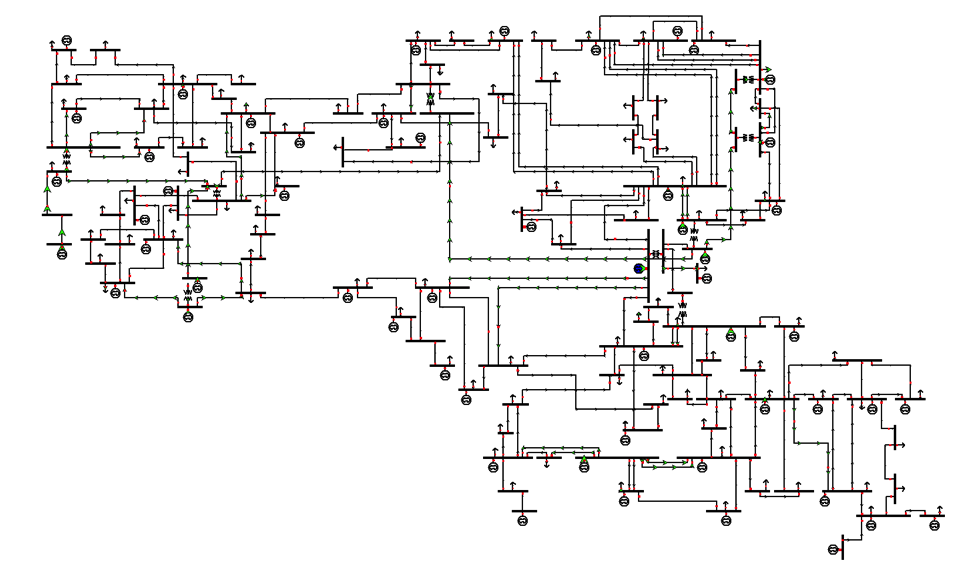
\includegraphics[width=1\textwidth]{pictures/IEEE118.png}
    \caption{IEEE118 grid scheme. \cite{grids:ieee118}}
    \label{fig:kundur}
\end{figure}

\subsection{COLMENA Integration \& Future Work}

We have seen two approaches that are useful in knowing how to simulate electrical grids with agents with multiple operating points (Case Study 1) and how to change parameters or other values during the simulation itself (Case Study 2). We propose a mixed solution that is inspired from the previous works but also tries to integrate itself into the existing COLMENA framework. The ANDES package as well as other tools simulate the grid up to a certain point while COLMENA is looking to simulate on a continuous time. For this we propose a combination of the frameworks in which COLMENA will call ANDES at irregular intervals of time and ANDES will run the dynamic simulation until a new steady-state point is reached. \\

For this, we define that agents can be available or locked. We consider that after a change of operating state the agent becomes active. This can be thought as being locked to the given operating point for a certain amount of time. After this time $t_{lock}$, the agent becomes available again.\\  

\begin{algorithm}
    \caption{TDS COLMENA-ANDES integration}
    \begin{algorithmic}[1]
    \State Initialize grid states $x$ to $x_0$ through Power Flow results.
    \State $t \gets 0$
    \While{not Stop}
        \While{No Agent is available}
            \State Run ANDES Normally
            \State $t \gets t + h$
        \EndWhile
        \State Go back to COLMENA
        \For{Agent in Agents that are available}
            \State Update Agent's operating point
        \EndFor
        \State $t \gets t + h$
    \EndWhile
    \State Finalize the result
    \end{algorithmic}
    \label{algo:COLMENAANDES}
\end{algorithm}

The proposed algorithm integrates COLMENA into the simulation. COLMENA selects the operating points for the different agents in the necessary step. It's also important to remark that there is a power flow simulation that is performed at the very beginning. This step ensures the grid starts the simulation from a feasible and stable state. Specifically it performs a steady state simulation that aims to find a simulation such that the device's states are constant, that is $f(x,y) = 0$.\\         

Performing the power flow simulation of a grid is considerably faster than doing a time domain simulation. Therefore, we could also consider a variation on the previous algorithm in which instead of computing the updated state in every new time step we compute the steady state directly and use it as. This simplification could be a possible alternative if COLMENA calls the simulation with enough time between each iteration so that we can consider that the grid achieves the steady state. Otherwise, the classic time domain simulation is more precise since it takes into account the dynamics of the electrical devices. \\

\addcontentsline{toc}{chapter}{References}
\printbibliography

\end{document}
